\documentclass[../notes.tex]{subfiles}
\graphicspath{{\subfix{../img/}}}
\begin{document}

\part{ECE358: Foundations of Computing}

\marginnote{Taught by Prof. Shurui Zhou}

\section{Admin and Preliminary Maths}

\subsection{Lecture 1}

Topics covered will include:
\begin{itemize}
	\item Graphs, trees
	\item Bunch of sorts
	\item Fancy search trees; red-black, splay, etc
	\item DP, Greedy
	\item Min span tree, single source shortest paths
	\item Maximum flow
	\item NP Completeness, theory of computation
	\item Blockchains??
	\item $ \Theta $ 
\end{itemize}

Solutions will be posted on the window of SF2001. Walk there and take a picture.

\subsubsection{Mark Breakdown}

\begin{table}[H]
	\centering
	\caption{Mark Breakdown}
	\begin{tabular}{|c|c|}
		\hline
		Homework x 5 & 25 \\
		Midterm (Open book) & 35 \\
		Final (Open book) & 40\\
		\hline
	\end{tabular}
\end{table}




\subsection{Complexities}


This lecture we talked about big O notation. For notes on this refer to my tutorial notes for ESC180, ESC190: \href{https://github.com/ihasdapie/teaching/}{https://github.com/ihasdapie/teaching/}


\begin{definition}
	Big O notation (upper bound)

	$ g(n) $  is an asymptotic upper bound for $ f(n) $ if:

	\begin{equation}
		O(g(n)) = \left\{f(n): \exists \quad c, n_0 \quad s.t. \quad 0 \le  f(n) \le  c\cdot g(n), \forall n \ge  n_o \right\}
		\label{eq:358:bigOh}
	\end{equation}
\end{definition}

\begin{proof}

	\textbf{What is the big-O of $ n! $ }?
	\begin{equation}
			n! \le n \cdot n \cdot n \cdot  n \ldots n = n^n \Rightarrow n! \in O(n^n) 
	\end{equation}
\end{proof}



\begin{definition}
	Big $ \Omega $  notation (lower bound)

	$ h(n) $  is an asymptotic lower bound for $ f(n) $ if:
	\begin{equation}
		\Omega(h(n)) =  \left\{f(n): \exists \quad {c, n_0} > 0 \quad s.t. \quad 0 \le c \cdot h(n) \le  f(n), \forall n \ge  n_o \right\}
		\label{eq:358:bigOmega}
	\end{equation}
\end{definition}

\begin{proof}

	\textbf{Find $ \Theta $ for $ f(n) \sum^n_i i $}.

	For this we will employ a technique for the proof where we take the right half of the function, i.e. from $ \frac{n}{2} \ldots n $ and then find the bound

	\begin{equation}
		\begin{split}
			f(n) &= 1 + 2 + 3 \ldots + n \\
			 &\ge \lceil \frac{n}{2} \rceil + (\left\lceil \frac{n}{2} \right\rceil + 1) + (\left\lceil \frac{n}{2} \right\rceil + 2) + \ldots n \quad \text{$ n/2 $ times} \\
			 &\ge \left\lceil \frac{n}{2} \right\rceil +   \left\lceil \frac{n}{2} \right\rceil + \left\lceil \frac{n}{2} \right\rceil +  \ldots \left\lceil \frac{n}{2} \right\rceil \\
			 &\ge \frac{n}{2} \cdot \frac{n}{2} \\
			 &= \frac{n^2}{4} \\
		\end{split}
	\end{equation}

	And therefore for $ c = \frac{1}{4} $  and $ n = 1 $ , $ f(n) \in \Theta(n^2) $ 
	
	
\end{proof}



\begin{definition}
	Big $ \Theta $  notation (asymptotically tight bound)

	\begin{equation}
		\Theta(g(n)) = \left\{ f(n) : \exists \quad c_1 c_2, n_0 \quad s.t. \quad 0 \le  c_1 g(n) \le  f(n) \le  c_2 g(n), \forall n \ge  n_o   \right\}
		\label{eq:358:bigTheta}
	\end{equation}
\end{definition}

\begin{proof}
	Prove that 

	\begin{equation}
		\sum^n_{j=1} i^k = \Theta(n^{k+1})
	\end{equation}

	First, prove $ O(f(n)) = O(n^{k+1}) $ 

	\begin{equation}
		\begin{split}
			f(n) = \sum^n_{j=1} i^k &= 1^k + 2^k + \ldots n^k \\
			 &\le n^k + n^k + \ldots n^k  \\
			 &= n^{k+1} \\
		\end{split}
	\end{equation}


	Next, prove $ \Omega(f(n)) = \Omega(n^{k+1}) $ 

	\begin{equation}
		\begin{split}
			f(n) = \sum^n_{j=1} i^k &= 1^k + 2^k + \ldots n^k \\
			 &= n^k + (n_1)^k + \ldots 2^k + 1^k = \sum^n_{i=1} (n-i+1)^k \\
			 &\ge   \frac{n}{2}^k * n \ge \frac{n^{k+1}}{2^k} = \Omega(n^{k+1}) \\
		\end{split}
	\end{equation}

	Therefore $ f(n) = \Theta(n^{k+1}) $ 
\end{proof}

Note that we may not always find both a tight upper and lower bound so not all functions have a tight asymptotic bound.







\begin{theorem}
	\textbf{Properties of asymptotes:} 

	Note: $\land $ means AND

	\textbf{Transitivity} \mn{The following applies to $ O, \Theta, o, \omega $ }
	\begin{equation}
		(f(n) = \Theta(g(n)) \land g(n) = \Theta(h(n))) \Rightarrow f(n) = \Theta(h(n))
		\label{eq:358:asymptotic_transitivity}
	\end{equation} 


	\textbf{Reflexivity}\mn{The following applies to $ O, \Theta $ }
	\begin{equation}
		f(n) = \Theta(f(n))
		\label{eq:358:asymptotic_reflexivity}
	\end{equation}
	
	\textbf{Symmetry}
	\begin{equation}
		f(n) = \Theta(g(n)) \iff g(n) = \Theta(f(n))
		\label{eq:358:asymptotic_symmetry}
	\end{equation}
	

	\textbf{Transpose Symmetry}

	\begin{equation}
		\begin{split}
			 f(n) &= O(g(n)) \iff g(n) = \Omega(f(n))  \\
			 f(n) &= o(g(n)) \iff g(n) = \omega(f(n))  \\
		\end{split}
		\label{eq:358:asymptotic_transpose_symmetry}
	\end{equation}

\end{theorem}


Runtime complexity bounds can sometimes be used to compare functions. For example, $ f(n) = O(g(n)) $ is like $ a \le b $

\begin{itemize}
	\item $ O \approx \le $
	\item $ \Omega \approx \ge  $ 
	\item $ \Theta \approx \approx  $ 
	\item $ o \approx < $; an upper bound that is \textbf{not}  asymptotically tight
	\item $ \omega > $ a lower bound that is \textbf{not}  asymptotically tight
\end{itemize}

Note that there is no trichotomy; unlike real numbers where we can just do $ a<b $, etc, we may not always be able to compare functions.

\begin{figure}[H]
	\centering
	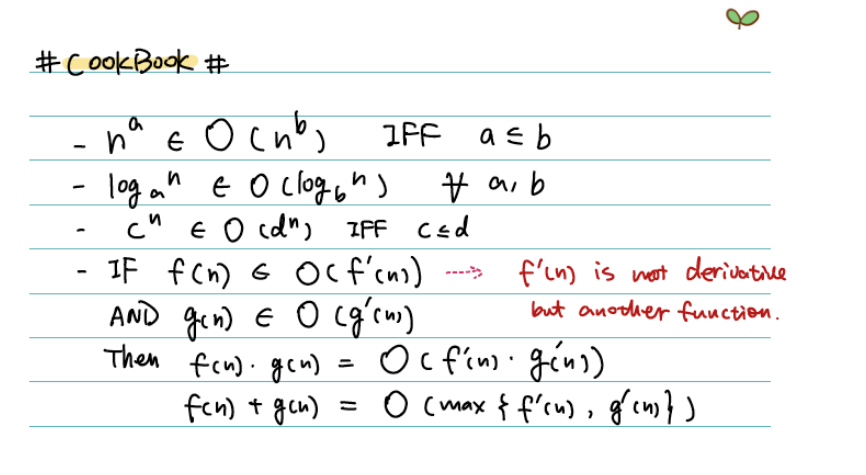
\includegraphics[width=0.8\linewidth]{img/image_2022-09-13-00-26-01.png}
	\caption{Complexity Cookbook}
	\label{fig:358:complexity_cookbook}
\end{figure}

\subsection{Lecture 3: Logs \& Sums}

\marginnote{
	Recall:
	\begin{equation}
		a = b^c \Leftrightarrow log_ba = c
	\end{equation}
}


\subsubsection{Functional Iteration}

$ f^{(i)}(n) $  denotes a function iteratively applied $ i $ times to value $ n $.

For example, a function may be defined as:
\begin{equation}
	f^{(i)}(n) = 
	\begin{cases}
		f(n) & \text{if } i = 0 \\
		f(f^{(i-1)}(n)) & \text{if } i > 0
	\end{cases}
	\label{eq:358:functional_iteration_1}
\end{equation}


Given \eqref{eq:358:functional_iteration_1} we see that 

\begin{enumerate}
	\item $ f(n) = 2n $ 
	\item $ f^{(2)}(n) = f(2n) = 2^2n$ 
	\item $ f^{(3}(n) = f(f^{(2)}(n)) = 2^3n$ 
	\vdots
	\item $ f^{(i)}(n) = 2^in $
\end{enumerate}


As an exercise we may look at an iterated logarithm function, 'log star`

\begin{equation}
	lg^*(n) = \min\{ i \ge  0 : lg^{(i)} n \le  1 \}
	\label{eq:358:iterated_logarithm}
\end{equation}

This describes the number of times we can iterate $ log(n) $ until it gets to $ 1 $ or smaller.

\begin{itemize}
	\item $ log^*2 = 1 $ 
	\item $ log^*4 = 2 = log^*2^2 = 1 + log^*2 = 2 $ 
		\vdots
	\item for practical reasons $ log^* $  doesn't really get bigger than $ 5 $. This is one of the slowest growing functions around.
\end{itemize}


\textbf{Summations \& Series} 

\begin{proof}

	Proof for a finite geometric sum:

	\begin{equation}
		\begin{split}
			\sum^n_{k=0} x^k &= S \\
			 S &= 1 + x + x^2 \ldots x^n  \\
			 xS &= x + x^2 + x^3 \ldots x^{n+1} \\
			 S &= \frac{1-x^{n+1}}{1-x} \\
		\end{split}
	\end{equation}
\end{proof}


\begin{equation}
	\sum^\infty_{i=1} x^i = \frac{1}{1-x} \quad \text{if } |x| < 1
	\label{eq:358:decreasing_geometric_series}
\end{equation}

\begin{equation}
	\sum^\infty_{k=0} kx^k = \frac{x}{(1-x)^2} \quad \text{if } |x| < 1
	\label{eq:358:geometric_series_2}
\end{equation}

\begin{proof}

	Begin by differentiating both sides over $ x $ 

	\begin{equation}
		\sum^\infty_{k=0} x^k = \frac{1}{(1-x)} \quad \text{if } |x| < 1
	\end{equation}

	\begin{equation}
		\sum^{\infty}_{k=0} kx^{k-1} = \frac{1}{(1-x)^2}
	\end{equation}

	And then multiply both sides by $ x $, therefore \eqref{eq:358:geometric_series_2} follows.
\end{proof}

\textbf{Telescoping Series} 

\begin{equation}
	\sum_{k=1}^{n} a_k - a_{k-1} = a_n - a_0
\end{equation}

\begin{proof}
	Write it out and cancel out terms
	\begin{equation}
		(a_1 - a_0) + (a_2 - a_1) \ldots (a_n - a_{n-1}) = a_n - a_0
	\end{equation}
	Therefore the sum telescopes
\end{proof}


Another telescoping series may be proved similarly:
\begin{equation}
	\sum^{n-1}_{k=1} \frac{1}{k(k+1)} \xrightarrow{math} \sum^{n-1}_{k=1} (\frac{1}{k} - \frac{1}{k+1}) 
	= 
	(1- \frac{1}{2}) + \ldots (\frac{1}{n-1} - \frac{1}{n}) = a_o - a_n
\end{equation}


\subsection{Lecture 4: Induction \& Contradiction}


\subsubsection{Induction}

The general steps for proving a statement by induction are:
\begin{enumerate}
	\item Basis
	\item Hypothesis
	\item Inductive step
\end{enumerate}

I.e. if the basis holds for some $ i $, i.e. $ 0, 1, 2, 3, 12, \ldots$ AND if we assume that the hypothesis holds for an arbitrary number $ k $, then we just need to prove that the inductive step follows, or that $ P(n+1) $ holds.

\begin{example}
	Prove that $ P(n) = 1+2+3+\ldots n = \frac{n(n+1)}{2} $ 
	\begin{proof}
		
	

	\begin{enumerate}
		\item Basis: $ P(0) = 0 = \frac{0(0+1)}{2} $
		\item Hypothesis (assume that it is true): $ P(k) = \frac{k(k+1)}{2} $
	\item Inductive step (need to prove $ P(k+1) = \frac{(n+1)(n+2)}{2} $ ): $ P(k+1) = \underbrace{1+2+\ldots+n}_{\frac{n(n+1)}{2}} + (n+1) = \ldots = \frac{n^2 + 3n + 2}{2} = \frac{(n+1)(n+2)}{2} $
	\end{enumerate}

	\end{proof}
	
\end{example}


\begin{example}
	Show that for any finite set $ S $, the power set $ 2^S $ has $ 2^{|S|} $ elements (that is, there are $ 2^{|S|} $ distinct subsets of $ S $  )\marginnote{The power set of a set $ S $ is the set of all subsets of $ S $ }

	\begin{proof}

		\begin{enumerate}
			\item Basis: 
				\begin{equation}
				n = 0, |S| = 0, |2^S| = 1 = 2^0 
				\end{equation}

				\begin{equation}
					n = 1, |S| = 1, |2^S| = 2 = 2^1
				\end{equation}
			\item Hypothesis: Assume that $ 2^S $ has $ 2^n $ elements when $ |S| = n $ 
			\item Inductive step: need to prove that when $ |S| = n+1, |2^S| = 2^{n+1} $ 

				Let $ B = S  \not \{a\}  $ for some $ a \in S $. 
				Now there are two types of subsets of $ S $; those that include $ a $ and those who do not include $ a $ 

				For subsets that do \textit{not} include  $ a $ , $ |2^{B}| = 2^{|B|} = 2^n $ , by the hypothesis.

				For subsets that do include $ a $, these sets are of size $ 2^B \cup \{a\}, which is  2^n  $ .

				Therefore the total number of subsets of $ S $ is $ 2^n + 2^n = 2^{n+1} $, as desired.
		\end{enumerate}
	\end{proof}
	
\end{example}

The same kind of argument can be applied to problems such as the \href{https://en.wikipedia.org/wiki/Tower_of_Hanoi}{Towers of Hanoi} and the tiling problem.


\subsubsection{Contradiction}
\begin{enumerate}
	\item Assume the theorem is false
	\item Show that the assumption is false (leads to a contradiction)
		\begin{itemize}
	\item Therefore the theorem is true
		\end{itemize}
\end{enumerate}

\begin{example}
	Prove that $ \sqrt{2}  $ is irrational
	\begin{proof}
		Assume that $ \sqrt{2}  $ is rational.

		Therefore we can write $ \sqrt{2}  $ as

		\begin{equation}
			\sqrt{2}  = \frac{a}{b}
		\end{equation}

		Where $ a, b $ \textbf{ have no common factors}.

		We can square both sides

		\begin{equation}
			2 = \frac{a^2}{b^2} \rightarrow a^2 = 2b^2
		\end{equation}

		Therefore $ a^2 $ is even. 

		Let $ a = 2c $ 

		\begin{equation}
			2^2 c^2 = 2b^2 \rightarrow b^2 = 2c^2
		\end{equation}

		Therefore $ b $ is even as well.

		This results in a contradiction since we assumed that $ a, b $ have no common factors, but our analysis shows that both would have to be even (and share a common factor of $ 2 $ ).
	\end{proof}
	
\end{example}


\subsection{Lecture 5: Recurrences}
Many recursive algorithms can be thought of as a divide-and-conquer approach where we break the problem into subproblems that are similar to the origianl but smaller in size, solve them resurisively, then combine them to create a solution to the original problem.


\begin{definition}
	A recurrence is a function defined in terms of:
	\begin{itemize}
		\item 1+ base cases
		\item Itself, with smaller arguments
	\end{itemize}
\end{definition}

For example, finding a Fibonacci number is a recurrence;

$ T(n) = T(n-1) + T(n-2) $ with some base cases.



\begin{example}
	\textbf{Mergesort} 

	Sorting $ [3,1,7,5] $ 

	\begin{enumerate}
		\item Divide: break into partitions: $ [[3, 1], [7, 5]] $ 
		\item Sort partitions: $[[1, 3], [5, 7]] $ 
		\item Create result array
		\item Compare: have two pointers to front of array
			\begin{itemize}
				\item compare 1, 5. 1 is smaller; $ result = [] \leftarrow 1 $ 
				\item Move ptr to left array (1, 3) ahead one. Compare 3, 5. 3 is smaller, so $ result = [3] \leftarrow 3 $ 
				\item One of the arrays is now empty so we can just append the rest
			\end{itemize}
		\item $ result = [1, 3, 5, 7] $ 
	\end{enumerate}
\end{example}


\begin{definition}
	Pseudocode for mergesort is given by:

	\begin{listing}[H]
	\begin{minted}{text}
	mergesort(A, p, r)
		if p < r
			q = [(p+r)/2]
			mergesort(A, p, q)  // N/2
			mergesort(A, q+1, r)  // N/2
			merge(A, p, q, r) // merge the sorted subarrays
	\end{minted}
	\end{listing}

	This mergesort partitions in half each time\mn{binary partitioning(?)}.

	In the worst case we will compare $ N-1 $ times, so $ O(N) $ worst case.

	Proving that merge sort is $ \Omega(N) $ 
	\marginnote{Here we're discussing not time complexity but rather the number of times we call mergesort}
	
\end{definition}

How much time does MergeSort take?


The time of mergesort is defined recursively as:
\begin{equation}
	T(N) = \begin{cases}
		O(1) & n = 1 \\
		T(N) = 2T(\frac{N}{2} + \Theta(N)
	\end{cases}
\end{equation}

\marginnote{Note that $ \Theta(N) $ is for the merge operation }

More generally we can find the runtime of a recurrence algorithm via
\begin{itemize}
	\item Recurrence trees
	\item Substitution
	\item Master theorem
\end{itemize}


\subsubsection{Recurrence Trees}
\begin{example}
Recurrence trees can be used to find the time complexity of mergesort.
\begin{figure}[H]
	\centering
	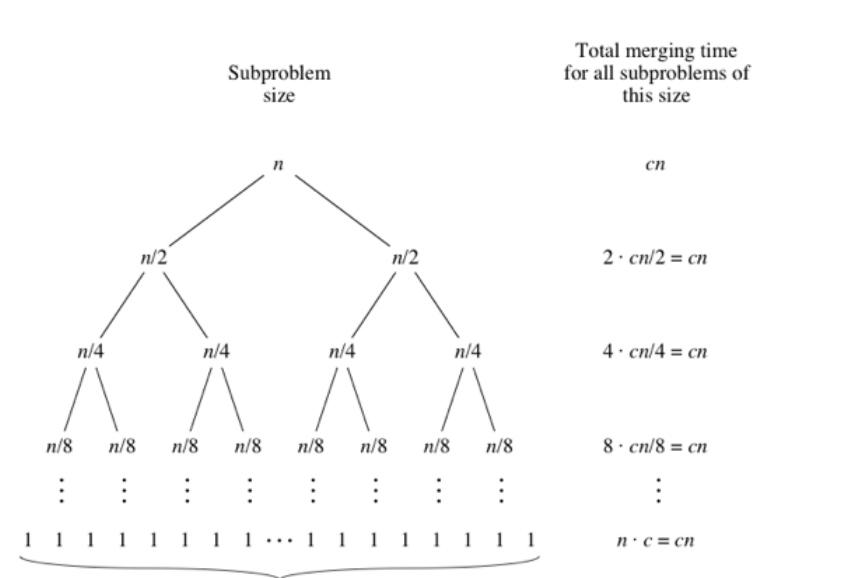
\includegraphics[width=0.8\linewidth]{img/image_2022-09-19-12-26-07.png}
\end{figure}

The height of the tree is $ \log N$ 

The total cost is the total cost per level times the number of levels, which is 

\begin{equation}
	N \cdot  logN
\end{equation}

So the complexity is $ O(N\log N) $ 
	
\end{example}

\subsubsection{Substitution}

\begin{enumerate}
	\item Guess the answer
	\item Apply induction
\end{enumerate}


\begin{example}
	Determine an asymptotic upper bound on $ T(n) = 2T(\left\lfloor \frac{n}{2} \right\rfloor ) + \Theta(n)$ 
	\begin{proof}

		This expression can be simplified since we don't care too much about floors or ceilings for asymptotic behaviour.

		\begin{equation}
			T(n) = 2T(\frac{n}{2}) + N
		\end{equation}

		Let's guess that the upper bound is $ O(n\log n) $ 

		Then, we need to prove that $ T(n) < C \cdot n \log n$  for some $ C > 0 $. Let's apply induction.

		\begin{enumerate}
			\item Basis: this is tricky since if $ n =1  $ we end up with $ T(1) \le  C \cdot 1 \cdot \log 1 = 0$ which cannot hold since that would just not make sense. Instead, observe that $ T(1) = 1 $, $ T(2) = 2T(1) + 2 = 4 $, $ T(3) = 2T(1) + 3 = 5  $, $ T(4) = 2T(2) + 4  \ldots$.

				So $ T(n) $ is therefore independent of $ T(1) $, so we can use two bases, $ T(2),T(3)$. Since $ T(2) \le  C * 2 \log 2 = 2C$, $ T(3) \le C \cdot \log  $ 
			\item Hypothesis: Assume that the upper bound holds for all possible $ m < n$, let $ m = \left\lfloor \frac{n}{2} \right\rfloor$ . This yields $ T(\frac{n}{2}) \le C \cdot  \left\lfloor \frac{n}{2} \right\rfloor \cdot  \log \left\lfloor \frac{n}{2} \right\rfloor $ 
			\item Inductive step: substitute hypothesis into recurrence yields 

				\begin{equation}
				 T(N) \le C \cdot ( C \cdot \left\lfloor  \frac{N}{2} \right\rfloor \cdot  \log \left\lfloor \frac{N}{2} \right\rfloor + N  = c N\log N - (1-c)N \le Cn\log n
				\end{equation}
		\end{enumerate}
		
	\end{proof}

	A few pitfalls to avoid is guessing $ T(n) = O(n) = c \cdot  n $ and so forth we would get

	\begin{equation}
		T(N) \le  2 C \cdot  \left\lfloor \frac{n}{2} \right\rfloor + n = cn+n = (c+1)n
	\end{equation}

	This would be wrong since we cannot change the constant to $ c+1 $; we have to prove it with exactly the hypothesis given.
	
\end{example}

\subsubsection{Master Theorem}

\marginnote{Proof is out of scope for the course}
\begin{definition}
	The master method applies to recurrences of the form 

	\begin{equation}
		T(n) = a T(\frac{n}{b}) + f(n) \qquad \text{where } a \ge 1, b >  1, f  \text{asymptotically positive}
	\end{equation}

	It distinguishes 3 common cases b comparing $ f(n)  $  with $ n^{\log_ba}$ 

	\begin{enumerate}
		\item If $ f(n) = O(n^{\log_ba - \varepsilon}) $ for some $ \varepsilon > 0 $, then $ T(n) = \Theta(n^{log_ba}) $ 
		\item If $ f(n) = \Theta(n^{\log_ba }) $, then $ T(n) = \Theta(n^{log_ba}\log n) $ 
		\item If $ f(n) = \Omega(n^{\log_ba + \varepsilon}) $ for some $ \varepsilon>0 $ and $ af(\frac{n}{b}) \le  c f(n) $ for some $ c < 1$, then then $ T(n) = \Theta(f(n)) $ 
	\end{enumerate}
\end{definition}


There are a few technicalities to be a ware of. 
In each example we compare $ f(n) $ with $ F = n^{\log_ba} $ and take the larger of each as the solution the recurrence. 
For the first case we note that $ f(n) $ must be \textit{polynomially} smaller than $ F $; i.e. it must be asymptotically smaller than $ F $ by some factor of $ n^\varepsilon $.
In the third case $ f(n)  $ must be greater than $ F $ as well as being polynomially larger and satisfy the regularity condition $ af(\frac{n}{b}) \le cf(n)$.
There are areas where the master theorem does not cover, for example a gap between cases 1, 2 where $ f(n) > F $ but is not polynomially larger. If $ f(n)  $ falls in one of these gaps or the regularity condition does not hold, the master method cannot be used to solve the recurrence.


\begin{example}

	What is the closed form of $T(n) = T(\frac{2n}{3}) + 1$ ?

	\begin{proof}
		a = 1, b = 2/3, f(n) = 1.

		\begin{equation}
			\log_ba = \log_{\frac{2}{3}} 1 = 0 
		\end{equation}

		\begin{equation}
			f(n) = \Theta(n^0)
		\end{equation}

		So
		\begin{equation}
			T(n) = O\log(n)
		\end{equation}
		
	\end{proof}
	


	
\end{example}








\section{Graphs}


\begin{definition}
A \textbf{graph} is a data structure comprised from set of vertices $ V $ and a set of edges $ E $, where each edge connects a pair of vertices.
A \textbf{directed graph (digraph)} is a graph where edges $ E $ have a \textit{direction}, i.e. an edge $ (u,v) $ is different from $ (v,u) $.
Conversely, an \textbf{undirected graph} is a graph where edges $ E $ do not have a direction.
\begin{figure}[H]
	\centering
	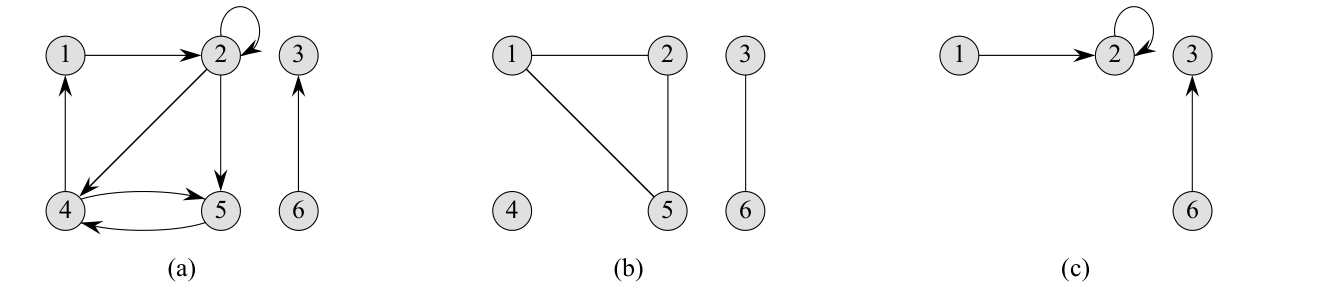
\includegraphics[width=0.8\linewidth]{img/image_2022-09-22-00-05-04.png}
	\caption{(a) directed graph, (b) undirected graph, (c) a subgraph of (a)}
\end{figure}

\end{definition}

Some conventions:

\begin{itemize}
	\item Edges are denoted by $ (u,v) $\mn{not $ \{u, v\} $  } where $ u,v \in V $
	\item If $ (u,v)$ is a edge in a directed graph, then $ (u,v) $ is incident from or leaves $ u $, and is incident to or enters $ v $ 
	\item If $ (u,v) $ is a edge a graph, then $ u$ , $ v $ are adjacent
	\item The \textbf{degree} of a vertex is the number of edges incident to it
	\item A \textbf{path} is a sequence of vertices $ (v_0, v_1, \ldots v_k) $ from from vertex to another such that each vertex is incident\mn{with the exception of start/end vertices} to the ones prior and after.
		\begin{itemize}
			\item If there exists a path from $ a $  to $ b $ then $ b $ is \textbf{reachable} from $ a $ and $ a $
			\item A path is \textbf{simple}  if no vertex is repeated
			\item A path forms a cycle if the first and last vertices are the same
		\end{itemize}
	\item A directed graph with no self-loops is \textbf{simple} 
	\item A graph with no simple cycles is acyclic
	\item An undirected graph is \textbf{connected} if there exists a path between any two vertices
	\item A directed graph is \textbf{strongly connected} if every vertex is reachable from every other vertex
	\item Two graphs $ V, V' $  are \textbf{isomorphic} if there exists a bijection\mn{$ f: V \to V' $, i.e. we can relabel the vertices of $ V $ to be those of $ V' $ and the two graphs would be identical   } between the vertices of the two graphs such that the edges are preserved
	\item Given graph $ G $,  $ G' = (V', E') $ is a \textbf{subgraph}  of $ G $  if $ V' \subseteq V $ and $ E' \subseteq E $
	\item Given a set $ V' \subseteq V $, the subgraph of $ G $ \textbf{induced} by $ V' $ is the graph $ G' = (V', E') $ where $ E' = \{ (u,v) \in E | u,v \in V' \} $
	\item Given an undirected graph, the \textbf{directed version} of $ G $ is $ G = (V, E') $  where $ (u,v) \in E' $ if and only if $ (u,v) \in E $. In other words we replace all undirected edges and replace them with their directed counterpart.
	\item The corollary can be applied to a directed graph to get the \textbf{undirected version} of $ G $.
	\item A \textbf{neighbor} of $ u $ in a directed graph is any vertex $ v $ such that $ (u,v) \in E $ where $ E $ is the set of edges for the undirected counterpart of the graph
	\item A \textbf{complete} graph is a graph where every pair of vertices are connected by an edge
	\item A \textbf{bipartite graph} is an undirected graph $ G $  in which it's $ V $ can be partitioned into two disjoint sets $ V_1, V_2 $ such that every edge $ (u,v) \in E $ connects a vertex in $ V_1 $ to a vertex in $ V_2 $ or vice-versa
	\item An acyclic undirected graph is a \textbf{forest}
	\item A connected acyclic undirected graph is a \textbf{free tree}. 
		\begin{itemize}
			\item A directed acyclic graph is often termed a DAG
		\end{itemize}
	\item A multi-graph is a graph where edges can be repeated and self-loops are allowed
	\item A hyper-graph is a graph where edges can connect more than two vertices
	\item The \textbf{contraction} of an undirected graph $ G $ by an edge $ e = (u,v) $ is a graph $ G' $  where $ V' = V - \{u,v\} \cup \{x\} $, where $ x $ is a new vertex. Then, for each edge connected to $ u, v$ the edges are deleted and then reconstructed with $ x $, effectively 'contracting` $ u ,v $  into a single vertex
\end{itemize}

In code graphs are commonly represented as adjacency lists or adjacency matrices. 
This was covered in ESC190, but for reference:

\begin{figure}[H]
	\centering
	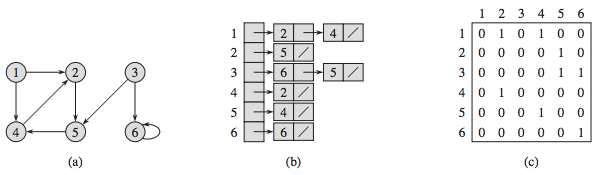
\includegraphics[width=0.8\linewidth]{img/image_2022-09-22-00-29-19.png}
\end{figure}

\begin{table}[H]
	\centering
	\caption{Time complexities of graph representations}
	\begin{tabular}{c|c|c|}
		\hline
		& adjacency list & matrix  \\
		Time & $ O(n) $ & $O(1)$ \\ 
		Memory & $ O(E) $ & $ O(n^2) $ 
	\end{tabular}
\end{table}












\section{Trees}

A \textbf{tree} is a common and useful subset of graphs
\begin{figure}[H]
	\centering
	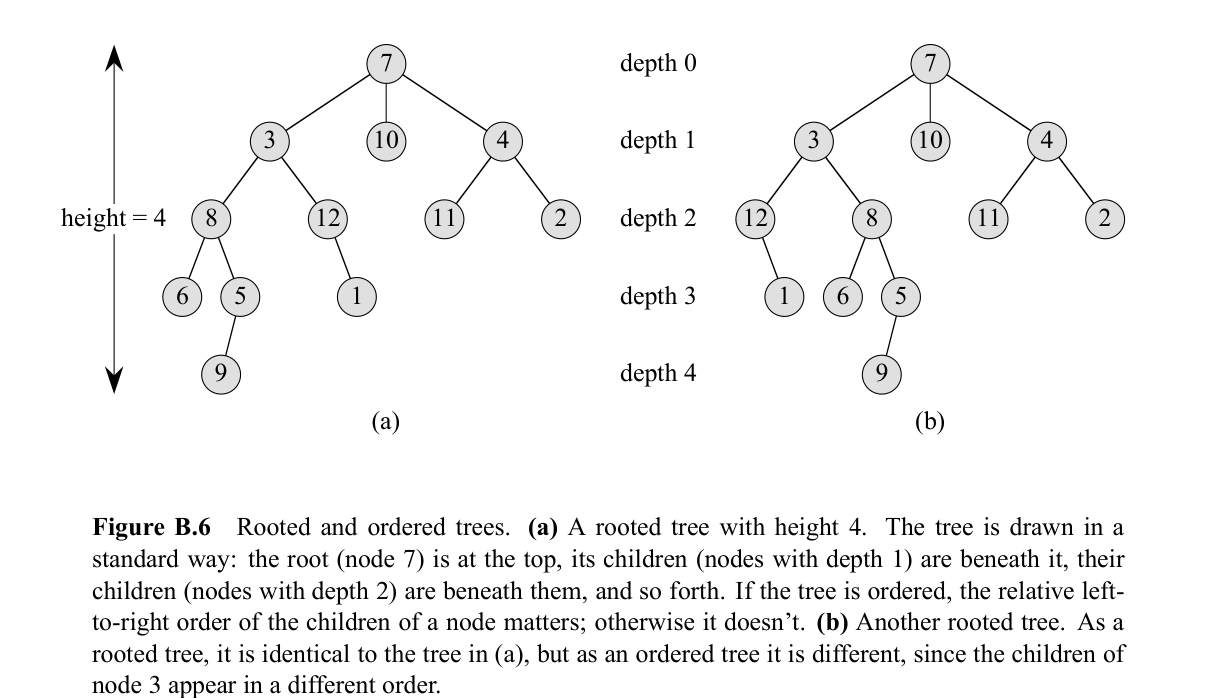
\includegraphics[width=0.8\linewidth]{img/image_2022-09-22-00-39-29.png}
\end{figure}
\begin{definition}
	A tree is a common subset of graphs, i.e. ones that are \textbf{connected, acyclic, and undirected}.
	This gives a few useful properties, i.e. the existence of a \textit{root} node, the parent-child relationship, and the existence of a unique path between any two nodes.
\end{definition}

Some conventions for trees

\begin{itemize}
	\item Depth of node: length from root to node
	\item Height length of longest path from node to leaf
	\item Degree of node: number of children. Binary trees have degree 2, n-ary tree has degree n
\end{itemize}

\begin{theorem}
	All of the following statements are equivalent for a tree $ T = (V, E) $:

	\begin{enumerate}
		\item $ \forall v \in V, v $ is a tree; all nodes in a tree are trees unto themselves.
		\item Every two nodes are connected by a unique path
		\item $ T $ is connected by if any edge is removed the resulting graph is disconnected
			$ T $ is connected and $ |E| = |V| - 1 $   
			$ T $ is acyclic and $ |E| = |V| - 1 $   
			$ T $ is connected but if a edge is added the resulting graph has a cycle
	\end{enumerate}



\end{theorem}






\section{Lecture 7, 8: Probability and Counting}

Most of the probability stuff is review from ECE286 so I'll be omitting most notes.


\begin{definition}
	Probability distribution $ Pr \left\{  \right\}  $: mapping from events of $ S $ to real numbers where

	\begin{enumerate}
		\item $ Pr \left\{ \emptyset \right\} = 0 $
		\item $ Pr \left\{ A \right\} \ge  0  \forall A \in S $
		\item $ Pr \left\{ S \right\} = 1 $
		\item $ Pr \left\{ A \cup B \right\} = Pr \left\{ A \right\} + Pr \left\{ B \right\} \forall A, B \in S $
	\end{enumerate}
\end{definition}
\marginnote{The complement of an event $ A $ is $ \overline{A} = S-A $, and the probability is $ Pr \left\{ \overline{A} \right\} = 1- Pr \left\{ A \right\}  $  } 

For any two events $ A, B $ we can define the triangle inequality
\begin{definition}
	$ Pr \left\{ A \cup B \right\} \le Pr \left\{ A \right\} + Pr \left\{ B \right\} $
\end{definition}


\begin{definition}
	Baye's thereom


	\begin{equation}
		Pr \left\{ A \mid B \right\} = \frac{Pr \left\{ B \mid A \right\} Pr \left\{ A \right\}}{Pr \left\{ B \right\}}
		= \frac{Pr \left\{ A \right\} Pr \left\{ B | A \right\} }{Pr \left\{ A \right\} Pr \left\{ B | A \right\} + Pr \left\{ \overline{A} \right\} Pr \left\{ B | \overline{A} \right\} }
	\end{equation}
	
\end{definition}


The expected value of a random variable is 

\begin{equation}
	E[X] = \int_{-\infty}^{\infty} x Pr \left\{ X = x \right\} dx
\end{equation}

And in the discrete case,
\begin{equation}
	E[X] = \sum_{x \in \mathbb{Z}} x Pr \left\{ X = x \right\}
\end{equation}


The variance is 

\begin{equation}
	Var[X] = E \left\{ \left( X - E[X] \right)^2 \right\} = E[X^2] - E^2[X]
\end{equation}

\marginnote{The \textbf{standard deviation, $ \sigma $, } is the positive square root of the variance.}




\section{Sorting}

\subsection{Heapsort}

Heapsort is a sorting algorithm that runs in $ O(nlog(n)) $ and sorts its elements in place by leveraging a \textit{heap}.
\marginnote{This should be review from ESC190}

\begin{definition}
A heap is a data structure that satisfies the \textit{heap property}. For a max heap, the value of a mode is at most the value of its parent and vice-versa for a min-heap. Heaps are commonly used to implement a priority queue because it offers a \texttt{pop\{min, max\}} operation in $ O(1) $ time and insertion in $ O(log(n)) $ time. Another reason for its use is it's ability to be represented as an array with \texttt{Parent(i) = floor(i/2)}, \texttt{Left(i) = 2i}\texttt{Right(i) = 2i+1} 

\end{definition}


The \texttt{MAXHEAPIFY} method is used to coerce heaps back into fulfilling the heap property by `bubbling down' nodes until the heap property is satisfied.
The intuition for this is that as long as the heap property is not satisfied\sn{which we can tell by looking at the node's children}, node $ i $ is exchanged for the largest of its' children. Since the heap property is now satisfied for $ i $ but not necessarily its' children, this heapify operation is then recursively called on the larger of $ i $'s children.

\begin{listing}[H]
\begin{minted}{text}
MAXHEAPIFY(A, i)
	l = LEFT(i)
	r = RIGHT(i)
	if l <=A.size and A[l] > A[i]
		largest = l
	else largest = i
	if r <= A.size and A[r] > A[largest]
		largest = r
	if largest != i
		swap A[i], A[largest]
		MAXHEAPIFY(A, largest)
\end{minted}
\end{listing}


The child sub-trees can have size of at most $ \frac{2n}{3} $ and so we can describe MAXHEAPIFY by the recurrence relation

\begin{equation}
	T(n) = \le  T(\frac{2n}{3}) + \Theta(1)
\end{equation}





This heapify operation can then be used to build a max heap from an array by calling heapify on all nodes that are not leaves. This is done by starting at the last node that has children and calling heapify on it. This is repeated until the root is reached. It can likewise be used to sort an array.



\begin{listing}[H]
\begin{minted}{text}
HEAPSORT(A)
for i = A.length -> 2,
	swap A[1], A[i]
	A.heapsize = A.heapsize - 1
	HEAPIFY(A, 1)
\end{minted}
\end{listing}



\subsection{Placeholder for Quick, counting, selection, and radix sort}

I'm going to skip these since these are fairly trivial and easily found online or in the textbook. I also didn't go to class.

\subsection{BSTs}
TODO: Notes on red-black trees, etc.


\section{Amortized Analysis}
\begin{definition}

	\begin{itemize}
		\item \textbf{Average cost}: mean across all inputs

			\begin{equation}
				\frac{1}{T-0} \int_{0}^{T} c(x) dx 
			\end{equation}
			
		\item \textbf{Expected cost}: expectation over all inputs w.r.t a probability distribution

			\begin{equation}
				\int_{0}^{T}   p(x) c(d) dx
			\end{equation}
			
		\item \textbf{Amortized Cost}: average cost over a \textit{sequence} of operations

			\begin{equation}
				\frac{1}{n} \sum_{i=1}^{n} c(\frac{1}{n})
			\end{equation}
	\end{itemize}

\end{definition}

The aggregate analysis method is simple and is as follows

\begin{enumerate}
	\item Given a function or operation $ f(x) $ and a sequence $ \left\{ x_1, x_2, \ldots x_n \right\}  $
	\item Determine the total cost of the sequence $ \sum_{i=1}^{n} c(x_i) \equiv T(n) $
	\item The amortized cost is $ \frac{T(n)}{n} $
\end{enumerate}

The complicated but more powerful way to deal with this is the accounting method.


\begin{enumerate}
	\item Declare a cost $ \hat{c} $ for each operation/function call
	\item Describe a procedure for how the cost will be allocated
	\item Assert a credit invariant, i.e. that the credit in an object must be greater than or equal to 0
	\item Prove the credit invariant
	\item Using the credit invariant argue why the credit never goes negative
	\item The amortized cost is $ O(\hat{c}) $
\end{enumerate}

Let's consider a contrived example.

\begin{example}
	Consider a data structure that has a cost of 


	\begin{equation}
		c(x) = \begin{cases}
			x & \text{if x is a power of 2} \\
			1 & \text{otherwise}
		\end{cases}
	\end{equation}

	Determine the amortized cost over the sequence $ \left\{ 1, 2, 3, 4, 5, 6, 7, 8, 9, 10 \right\} $

	The aggregate method for solving this problem is trivial; simply compute the summation to find

	\begin{equation}
		\sum_{x=1}^{n} c(x) = \ldots (2n-1) \leq 3n
	\end{equation}

	What's more interesting is how we may apply the accounting method

	\begin{enumerate}
		\item Let cost $ \hat{c} = 3 $
		\item If $ x $ is not a power of 2, uses $ 1 $ to pay for the operation and store the remaining $ 2 $
		\item If $ x $ is a power of 2, store $ 2 $ in credit and use $ x $ from previous iterations to pay for the operation
		\item (Steps 3, 4, 5) Prove the credit invariant. When $ x = 2^m $ all elements $ \in (2^{m-1}, 2^{m}] $ have $ 2 $ stored. The math can be a little handwavy but just draw out the ranges and show base cases etc.
		\item And the amortized cost is $ O(\hat{c}) = O(3) = O(1)$
	\end{enumerate}

\end{example}

What amortized cost is really telling us is that the cost of all operations as a whole is never larger than some value, though on the individual level it may fluctuate a little bit.

\begin{equation}
	\frac{1}{n} \sum_{i=1}^{n}  \hat{c} \ge \frac{1}{n} \sum_{i=1}^{n} c(x_i)  \qquad \forall n
\end{equation}

We can think of this is that the cumulative work stored in the data structure (amortized) being an upper bound on the actual cost.

\begin{equation}
	\frac{1}{n} \sum_{i=1}^{n}  (\hat{c} - c(x_i)) \ge  0 \qquad \forall n
\end{equation}



The credit invariant is used to prove the above inequality.


\marginnote{
	If $ c(x_i) \le  \hat{c}$ then we good and can store anything left over
	If $ c(x_i) >  \hat{c}$ then we need to use credit from previous iterations

	And the credit invariant is used to argue that we never use too much credit.
}

\begin{example}
	Consider a FIFO queue implemented using two stacks $ S_{in}, S_{out} $. The stacks have the operations \texttt{Push(Q, x)} (pushes x onto $ S_{in} $), \texttt{copy(Q)} (pops all elements from $ S_{in} $ and pushes onto $ S_{out} $), and \texttt{pop(Q)} (calls copy and then pops off $ S_{out} $)
\end{example}




\begin{table}[ht]
	\centering
	\begin{tabular}{|c|c|c|}
		operation & actual cost & amortized cost \\
		push & $ O(1)$ & $ O(1) $\\
		copy & $ O(n)$ & $ O(1) $\\
		pop & $ O(n) $&$ O(1) $ 
	\end{tabular}
\end{table}

\begin{itemize}
	\item Push: $ 1 $ pays for push onto $ S_{in} $
	\item $ 2 $ pays for the eventual copy
	\item $ 1 $ pays for the pop from $ S_{out} $
\end{itemize}

The credit invariant is therefore

\begin{enumerate}
	\item Elements in $ S_{in} $ have $ 3 $ in stored credit
	\item Elements in $ S_{out} $ have $ 1$ in stored credit
\end{enumerate}

The amortized cost of each operation is $ O(1) $ for all


\begin{example}
	Consider a sequence of stack operations on a stack which never exceeds $ k $ elements. After $ k $ operations, we copy the stack
\begin{table}[ht]
	\centering
	\begin{tabular}{|c|c|c|}
		operation & actual cost & amortized cost \\
		push & $ O(1)$ & $ O(1) $\\
		pop & $ O(1) $&$ O(1) $ \\
		copy & $ O(n)$ & $ O(1) $
	\end{tabular}
\end{table}


\begin{proof}
	

\begin{enumerate}
	\item Let cost = 2. Push: pay 1, store 1. Pop: pay 1, store 1, Copy: pay k
	\item credit invariant holds in stack because the number of credit stored on the stack equals the number of operations since the last copy. Since after each operation +1 is stored, then since the stack never has more than k elements after k operations we will have k stored and can therefore pay for the copy
\end{enumerate}


\end{proof}
\end{example}




\subsection{Skewed Heaps}

Consider a \textit{skewed heap} data structure which implements a \texttt{SkewHeapMerge} operation for merging heap-ordered trees by merging the rightmost paths of two trees without keeping any explicit balance conditions.
Good performance of skewed heaps is guaranteed by a rebalancing step which swaps all the left and right children of nodes along the rightmost path (except for the last one).
Since there is no balance condition the trees won't have $ O(\log n) $ worst case performance but they do have good amortized performance.


\begin{codebox}
\li \Procname{$\proc{SkewHeapMerge}(h, h')$}
\li \If $ h  \isequal NIL $\Then 
\li \Return $ NIL $ \End
\li \If $ h'  \isequal NIL $ \Then 
\li \Return $ NIL $ \End
\li \If $ h.key  \le h'.key $ \Then 
\li \Return $ \proc{SkewHeapMerge}(h', h) $ \End
\li $ h.right \gets \proc{SkewHeapMerge}(h.right, h') $
\li SWAP($ h.left, h.right $)
\li \Return h
\end{codebox}


\begin{example}
	Show that a \texttt{SkewedMeapMerge}, \texttt{Insert}, and \texttt{DeleteMin} uses amortized $ O(\log_2 n) $ time.

	\begin{enumerate}
		\item Allocate $ \hat{c}=c\log(n)$ per operation (since we want to prove that it's $ O(\log n) $ amortized)
		\item Define $ WT(x)$ as the number of nodes in the subtree rooted at x. Define a heavy node as a node with $ WT(x) \ge  WT(x.parent)$. Note that this doesn't include the root. A light node is exactly the opposite.
			\begin{itemize}
				\item If all nodes on the rightmost path are light, then the cost of $ \proc{SkewHeapMerge} $ is minimized
				\item Define a misplaced node as a heavy node on the rightmost path
			\end{itemize}

			Find the number of light nodes on any path from the root to the leaf.


	\end{enumerate}




\end{example}


\section{Minimum Spanning Trees}

\begin{definition}
	A minimum spanning tree is an acyclic subset of edges in a graph which connects all the vertices and has the minimum total weight\mn{i.e. sum of edge cost}
\end{definition}

Two common algorithms for solving the minimum spanning tree problem are Kruskal's algorithm and Prim's algirthm.
They are similar in that they both attempt to greedily add edges to the minimum spanning tree, but whereas Kruskal's algorithm grows a forest by adding the least weight edge in the graph that connects two distinct components, Prim's algorithm grows a single tree by adding the least-weight edge connecting the tree to a vertex outside fo the tree.


\begin{definition}
	\textbf{Terminology} 

	\begin{itemize}
		\item \textbf{Cut $ (S, V-S) $} is a partition of $ V $\mn{see it as dividing $ V $ into two new sets $ S, S-V $} 
		\item A cut \textbf{respects} a set $ A $ if no edge crosses the cut
		\item A \textbf{light edge} is the edge crossing a cut with the minimum weight
		\item A \textbf{safe edge} is any light edge crossing a cut $ S, V-S $ of $ G $ that respects the MST $ A $
	\end{itemize}
\end{definition}



\begin{codebox}
\Procname{$\proc{MST-Kruskal}(G, w)$}
\li $ A = \{0\}  $
\li \For each vertex $ v \in G.V $ \Do
\li 	$\proc{make-set}(v)$
\li 	sort $ G.E $ by weight $ w $ in nondecreasing order
\li \For each edge $ (u, v) \in G.E $ \Do
\li \If $ \proc{find-set(u)} \neq \proc{find-set}(v)$ \Then
\li $ A = A \cup \{(u, v)\}  $
\li $ \proc{union}(u,v) $ \End \End \End
\li \Return $ A $
\end{codebox}


In summary Kruskal's algorithm adds edges $ (u,v) $to the MST in non-decreasing order of weight, \textit{if} $ (u,v) $ do not belong to the same tree (as to prevent creating a cycle).
Note: The runtime of these algorithms can be improved using a priority queue on the edge weights. However if the graph is dense ($ E = V^2 $) an array can be better an array can be better

\begin{codebox}
\Procname{$\proc{MST-Prim}(G, w, r)$}
\li \For each vertex $ u \in G.V $ \Do
\li u.key = $\infty$
\li u.$\pi $  = NIL \End
\li $  Q = G.V $
\li \While $ Q \neq  \{0\}  $ \Do
\li u = \proc{Extract-Min}(Q)
\li \For each vertex $ v \in G.Adj[u] $ \Do
\li u.key = $w(u,v)$
\li u.$\pi $  = u \End \End \End
\end{codebox}

Prim's algorithm builds a MST set $ A $ that always forms a single tree. Each step adds a light edge to $ A $ that connects it to an isolated vertex. Since this only adds edges that are safe for $ A $ and $ A $ will eventually contain all vertices in $ V $, $ A $ forms a minimum spanning tree.

\section{Shortest Paths}

Common algorithms for solving the shortest path problem are Dijkstra's algorithm, Bellman-Ford's algorithm, and A*.

Dijkstra's algorithm and A* were discussed in ESC190 and such will not be discussed here. Bellman-Ford's algorithm, unlike Dijkstra, can handle negative weight edges\mn{though still fail to produce a shortest path as long as no negative-weight cycles are reachable, but can detect and report its existence.}

\begin{definition}
	\textbf{Relaxation} 

	For each vertex $ v \in V $, we maintain a \textit{shortest path estimate} $ v.d $ describing the upper bound on the weight of a shortest path from source to $ v $, i.e. $ s \rightsquigarrow v $. The initial state of $ v.d $ will just be $ \infty $

	\marginnote{$ \pi $ denotes the predecessor of a vertex in a shortest path from $ s $ to $ v $}
	\begin{codebox}
	\Procname{$\proc{initalize-single-source}(G,s)$}
	\li \For each $ v \in G.V $ \Do
	\li $ v=d = \infty $
	\li $ v.\pi = NIL $ \End
	\li $ s.d = 0 $
	\end{codebox}

	\textit{relaxing} an edge $ (u,v) $ means to check if the shortest path to $ v $ so far can be improved by going through $ u $, and updating $ v.d, v.\pi $ if so.
	\begin{figure}[H]
		\centering
		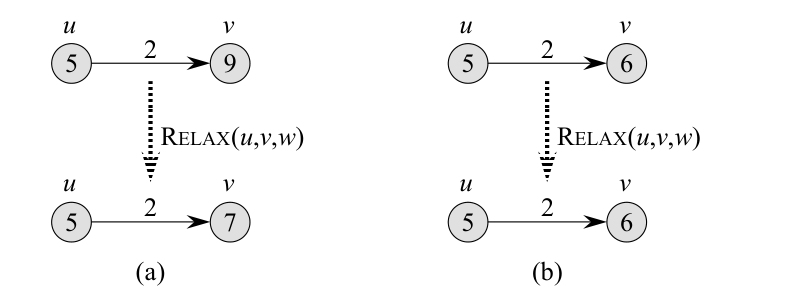
\includegraphics[width=0.8\linewidth]{img/image_2022-11-23-21-46-25.png}
		\caption{Relaxing an edge}
	\end{figure}

	\begin{codebox}
	\Procname{$\proc{relax}(u,v,w)$}
	\li	\If $ v.d > u.d + w(u,v)$ \Then
	\li	$ v.d = u.d + w(u,v) $
	\li	$ v.\pi = u $ \End
	\end{codebox}
\end{definition}

\marginnote{All of the presented algorithms use only $ \proc{relax} $ to change shortest-path estimates and predecessors. I'll also include the Dijkstra algo using $ \proc{relax} $ later as well.}

An issue with relaxation-based algorithms is that order matters; continuing to relax in a graph with negative weight cycles can cause an infinite loop, and a poor choice of order can lead to many unnecessary relaxations.
Bellman-Ford proposes proposes to label edges $ E $ in a topological order $  e_1 ... e_n$ and then relax them in that order $ |V| - 1 $ times.


\begin{definition}

	\textbf{Bellman-Ford Algorithm}
\begin{codebox}
\Procname{$\proc{bellman-ford}(G,w,s)$}
\li \proc{initalize-single-source}(G,s)
\li \For $ 1 \leq i \leq |G.V| - 1 $ \Do
\li \For each edge $ (u,v) \in G.E $ \Do
\li \proc{relax}(u,v,w) \End \End
\li \For each edge $ (u,v) \in G.E $ \Do
\li \If $ v.d > u.d + w(u,v)$ \Then
\li \Return \textbf{FALSE} \End \End
\li \Return \textbf{TRUE}
\end{codebox}
	
\end{definition}

The algorithm makes $ |V| - 1 $ passes over the graph, attempting to relax each edge $ |V| - 1 $ times.
Briefly we can see that the algorithm is correct by observing that the longest acyclic path in a graph with $ |V| $ vertices has length $ |V| - 1 $. And the algorithm maintains the invariant that the $ i$-th pass $ v.d $ is at most the weight of every path from $ s \rightsquigarrow v   $ using at most $ i $ edges. So by the $ |V| - 1$-th pass each edge is maximally relaxed, i.e. $ v.d = \delta(s,v) $ for all $ v \in V $, where $ \delta(u,v)$ denotes the actual shortest path weight

It then checks for a negative weight cycle reachable from the source, the proof for how this works can be found in CLRS Pg. 653\mn{But more or less the approach is to build a contradiction around how the sum of edge weights in a negative cycle is $ \le  0  $ and the conditions on $ v.d $ being equal to $ u.d + w(u, v) $}

In scenarios where we are working with DAGs we can use a topological sort to order the edges and relax them in that order -- which would result in a linear time algorithm $ \Theta(V+E) $. There are no negative-weight cycles possible in a DAG so shortest paths will always be well-defined


\begin{codebox}
\Procname{$\proc{DAG-bellman-ford}(G,w,s)$}
\li sort $ G.V $ topologically
\li \proc{initalize-single-source}(G,s)
\li \For each vertex $ u \in G.V $ taken in topological order \Do
\li \For each vertex $ v \in G.Adj[u] $ \Do
\li \proc{relax}(u,v,w) \End \End
\end{codebox}

Recall: topological ordering of DAG is a linear ordering of its vertices such that if $ u \rightsquigarrow v $ then $ u $ comes before $ v $ in the ordering, i.e. a graph traversal such that each node $ v $ is visited only after all its dependencies are visited.
An algorithm for topologically sorting a graph is just DFS with a colouring concept; WHITE for unvisited, GREY for visiting, and BLACK for visited. Time is simply a shared variable that increments for each call to DFS.
The starting time of a vertex is the time when it is first discovered, and the finishing time is the time when it is colored black. The topological ordering is the reverse of the finishing times.


\begin{codebox}
\Procname{$\proc{topological-sort}(G)$}
\li call DFS(G) to compute finishing times f[v] for each vertex v
\li as each vertex is finished, insert it onto the front of a linked list
\li \Return the linked list of vertices
\end{codebox}



Dijkstra's algorithm is then just a special case of the Bellman-Ford algorithm for a graph with no negative edge weights that relaxes greedily edges radially outwards from the source.


\begin{codebox}
\Procname{$\proc{dijkstra}(G,w,s)$}
\li \proc{initalize-single-source}(G,s)
\li $ S = \emptyset $
\li $ Q = G.V $
\li \While $ Q \neq \emptyset $ \Do
\li $ u = \proc{extract-min}(Q) $ (min on $ v.d $)
\li $ S = S \cup \{u\} $
\li \For each $ v \in G.Adj[u] $ \Do
\li \proc{relax}(u,v,w) \End \End
\end{codebox}



















\section{Splay Trees}

Consider the weight dictionary problem where we want to maintain a set of keys $ K = \{k_1, k_2 \ldots k_n \}  $ with associated values $ V = \{v_1, v_2 \ldots v_n \}$   and access frequencies $ W = \{w_1, w_2, \ldots w_n \}  $ and we want to access high-access-frequency item faster than low-frequency items without sacrificing efficiency on $ \proc{insert} $, $ \proc{search} $, and $ \proc{delete} $.
If no insert/delete operations are needed across the tree during runtime one can build the static optimal search tree i.e. the one that minimizes $ P = \sum_i w_i d_i $ where $ w_i $ is the weight of a path and $ d_i$ be the depth of node $ x_i $ ahead of time in $ O(n^3) $ with DP.
To motivate the study of splay trees, let's think of the case where we would want to remove from the BST and have different access frequencies during runtime; a more challenging problem.
A data structure that achieves an amortized time within a constant multiple of the theoretic lower bound is the \textbf{splay tree}; a self-organizing data structure, or one that moves $ x $ closer to the entry point (in a BST the root) whenever $ x $ is accessed.

\begin{definition}
	A splay tree is an ordered binary tree that satisfies

	\begin{itemize}
		\item every element in the left subtree of $ x $ is $ \leq $$ x $
		\item every element in the right subtree of $ x $ is $ \ge  $$ x $
	\end{itemize}

	Across which we can perform the $ \proc{splay} $ procedure

	\begin{figure}[H]
		\centering
		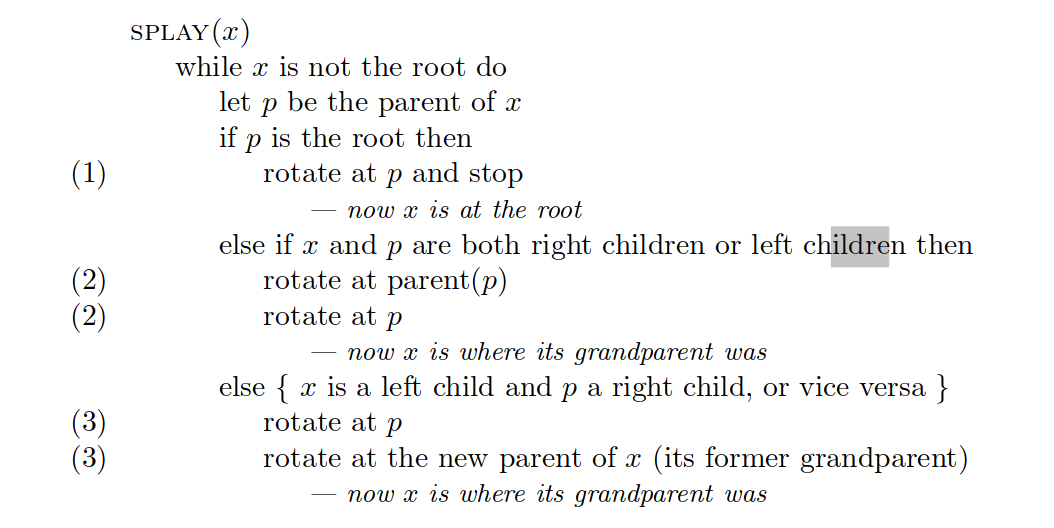
\includegraphics[width=0.8\linewidth]{img/image_2022-11-25-20-07-14.png}
	\end{figure}

$ \proc{splay} $ is a procedure that moves $ x $ to the root of the tree by rotating $ x $ and it's parent. There are a maximum of $ \frac{h}{2} $ steps or $ h $ rotations if the height of node $ x $ is $ h $ (Each step in $ \proc{splay} $ is actually two rotations)

	The other BST operations are therefore implemented as follows

	\begin{itemize}
		\item \textbf{$ \proc{locate}(x) $}: search for $ x $ in the tree and then call $ \proc{splay} $ on $ x $
		\item \textbf{$ \proc{insert}(x) $}: insert $ x $ into the tree as a leaf and then call $ \proc{splay} $ on the newly inserted $ x $
		\item \textbf{$ \proc{delete}(x) $} : Delete an element as usual. Leaf nodes can simply be removed; internal nodes are replaced by their in-order successor and then the successor is removed. Then call $ \proc{splay} $ on the parent of the deleted node.
	\end{itemize}






	\marginnote{Note that there is no explicit balance condition and as such the worst-case complexity can be $ O(n) $ but the \textit{amortized} complexity of each operation is $ O(log(n)) $}

\end{definition}

This splay operation causes items that are accessed most frequently to move closer to the root.

Definitions:
\begin{proof}
	Prove that $ \proc{splay} $ has an amortized cost of $ O(log(n)) $.

	\begin{itemize}
		\item Let $ \proc{WT}(x) $ be the weight of node $ x $, i.e the number of nodes in the subtree rooted at $ x $ including $ x $ itself.
		\item Let $ \proc{rank}(x) = \log \proc{WT}(x) $ 
	\end{itemize}


	Credit invariant: assert that there are always $ \proc{rank}(x) $ credits on $ x $, $ \forall x \in \text{tree} $. 1 credit will be charged in each rotate operation and only $ O(\log n) $ credits are needed in addition to maintain this invarient.


	Claim: for each step in the splay operation the number of additional credits is at most $ 3(\proc{new rank}(x) - \proc{old rank}(x))$ and maybe one more for the last step; any other credits can be taken from the tree.
	Consider the rank of $ x $ as the splay operation proceeds; $ \proc{rank}_0, \proc{rank}_1, \proc{rank}_2, ... \proc{rank}_k $.
	Therefore the total number of credits needed is 

	\begin{equation}
		 1 + 3(\proc{rank}_k - \proc{rank}_{k-1} \ldots 3(\proc{rank}_1 - \proc{rank}_0)
	\end{equation}

	Cancelling out terms,

	\begin{equation}
		 =  1 + 3(\proc{rank}_k - \proc{rank}_0)
	\end{equation}


	Since $ \proc{rank}_k = \log \proc{WT}(x) $, 

	\begin{equation}
		 1 + 3(\proc{rank}_k - \proc{rank}_0) \le  1 + 3 \log n
	\end{equation}


	Now let's analyze it with respect to the three rotation cases in $ \proc{splay} $; 
	\begin{enumerate}
		\item if $ x $'s parent is the root
		\item if $ x $ and its parent are both right or left children
		\item or if $ x $ is a left child and its parent is a right child or vice versa
	\end{enumerate}

	\begin{figure}[H]
		\centering
		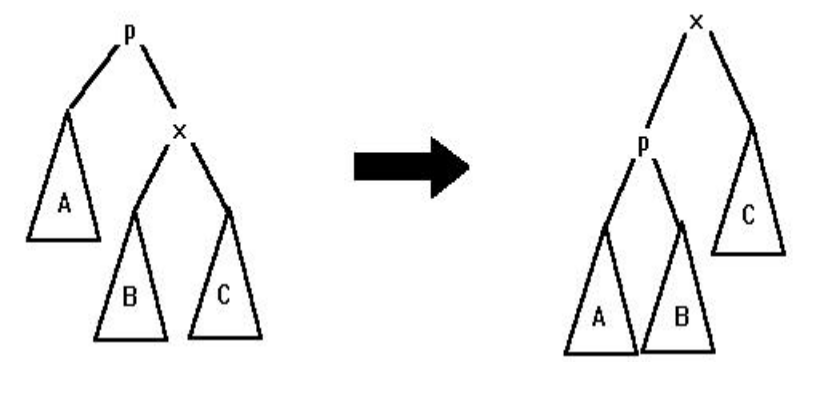
\includegraphics[width=0.8\linewidth]{img/image_2022-11-25-22-19-09.png}
		\caption{Case 1: $ x $'s parent is the root}
	\end{figure}

	This becomes a case of just counting the new and old ranks of $ x $ and its parent $ p $



	\begin{equation}
		\proc{old rank}(x) = \log (1 + |B| + |C|) \le  \proc{new rank}(x) = \log (2 + |B| + |C| + |A|)
	\end{equation}

	\begin{equation}
		\proc{old rank}(p) = \log (2 + |A| + |B| + |C|) \ge  \proc{new rank}(p) = \log (1 + |A| + |C|)
	\end{equation}

	$ p $ can only decrease in rank. $ x $ already has $ \proc{old rank}(x) $ credits, so we only need $ \proc{new rank}(x) - \proc{old rank}(x) $, which is  only 1/3 of the allocated credits. One more credit may be used to pay for the rotation, which can be taken from the +1 taken for the last step.



	
	
	\begin{figure}[H]
		\centering
		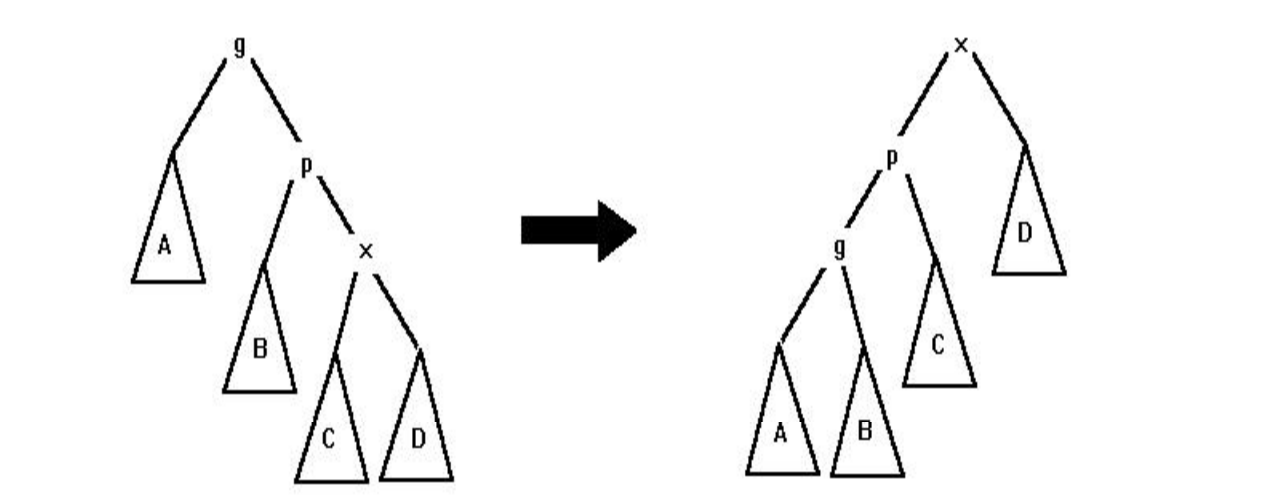
\includegraphics[width=0.8\linewidth]{img/image_2022-11-25-23-34-53.png}
		\caption{Case 2: $ x, p $ both left or right children}
	\end{figure}

	We have

\begin{equation}
	\proc{old rank}(x) + \proc{old rank}(p) + \proc{old rank}(g)
\end{equation}

Available and we need

\begin{equation}
	\proc{new rank}(x) + \proc{new rank}(p) + \proc{new rank}(g)
\end{equation}


Some math can be done to find that this is still bounded by our claim, i.e. $ 1 + 3(\proc{new rank}(x) - \proc{old rank}(x)) $


Here are the screenshotted notes (since I don't want to write it out)


\begin{figure}[H]
	\centering
	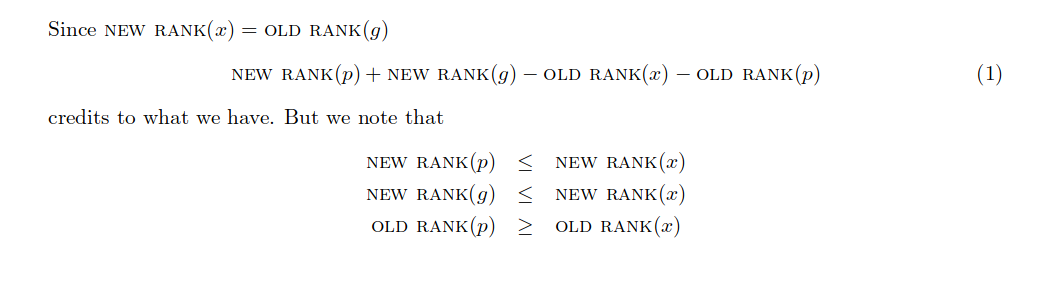
\includegraphics[width=0.8\linewidth]{img/image_2022-11-25-23-39-53.png}
\end{figure}


\begin{figure}[H]
	\centering
	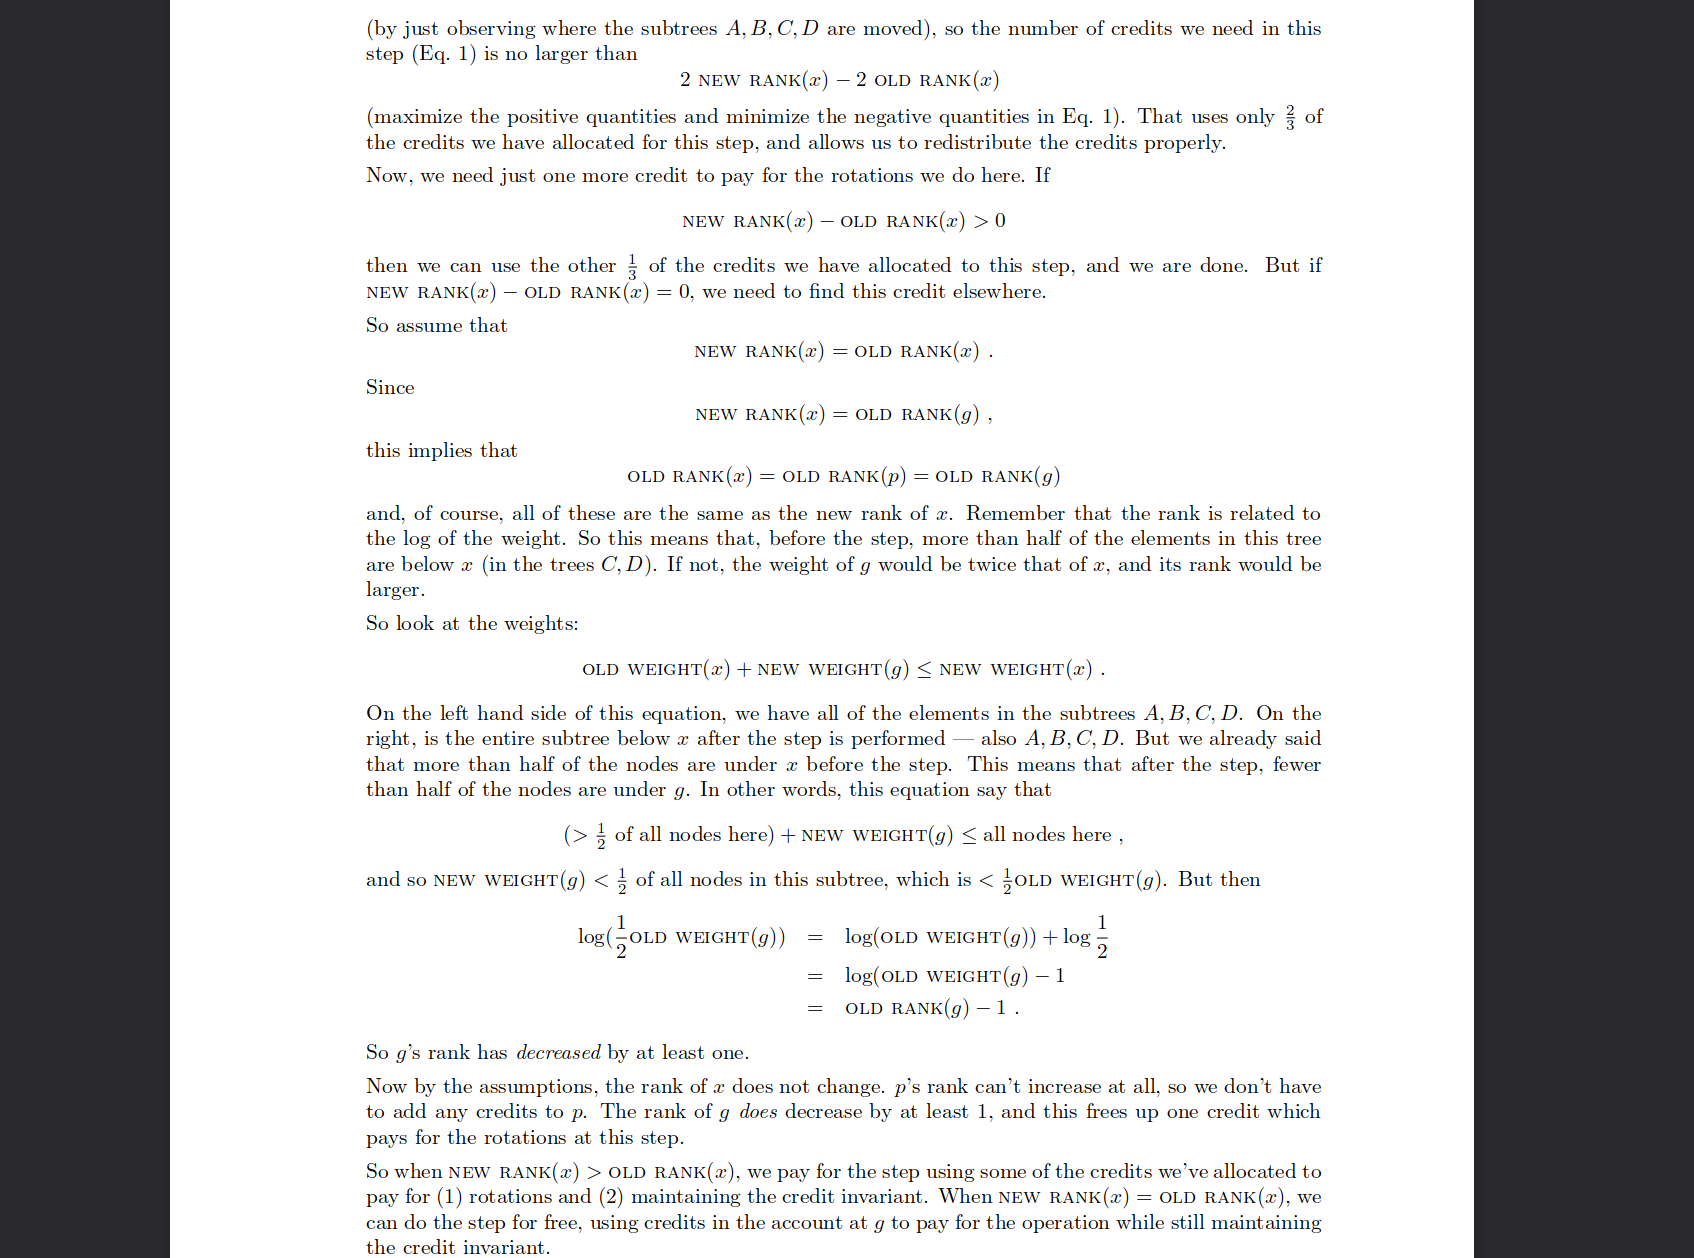
\includegraphics[width=0.8\linewidth]{img/image_2022-11-25-23-40-04.png}
\end{figure}


A very similar proof follows for case 3. 
\begin{figure}[H]
	\centering
	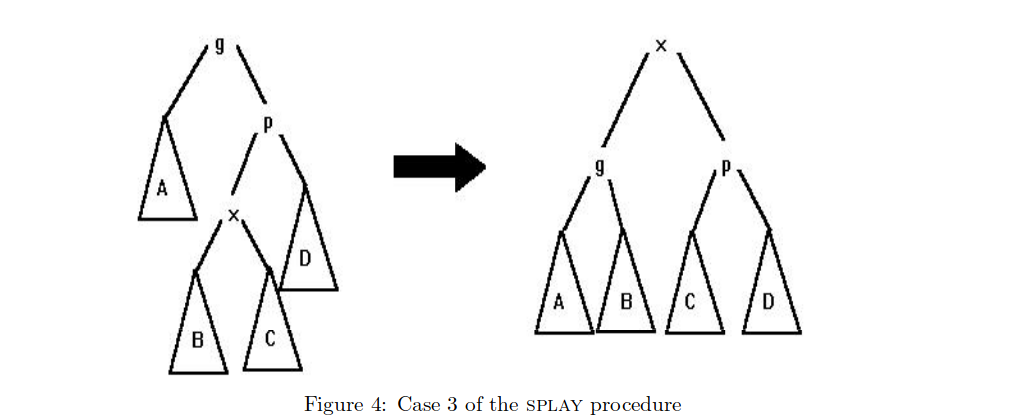
\includegraphics[width=0.8\linewidth]{img/image_2022-11-25-23-40-31.png}
	\caption{Case 3}
\end{figure}

One edge case to consider is when the new rank of $ x $ is the same of the old rank $ x $. This can be solved by considering the ranks of $ g $ and $ p $

\begin{figure}[H]
	\centering
	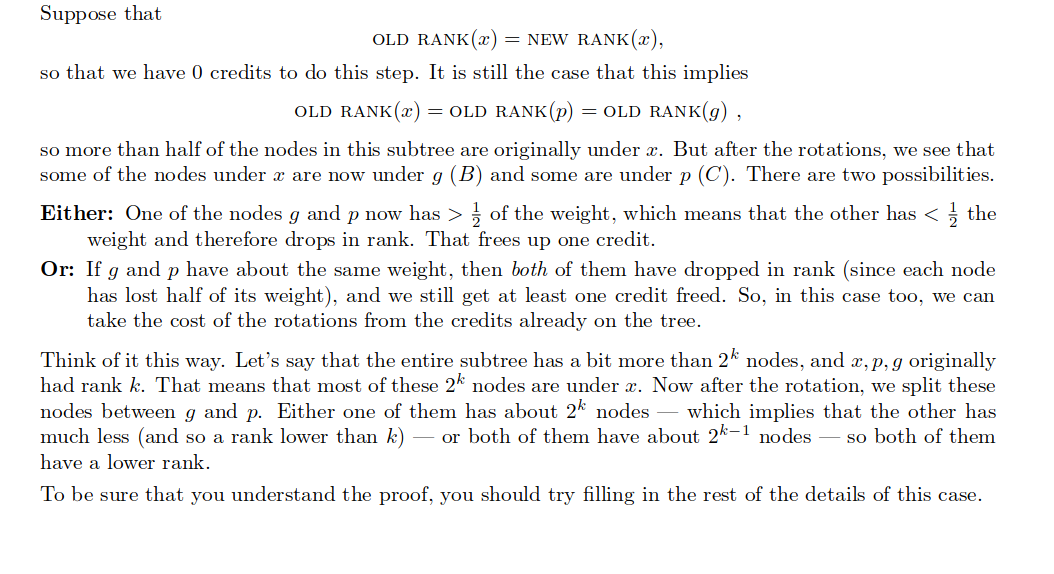
\includegraphics[width=0.8\linewidth]{img/image_2022-11-25-23-41-12.png}
\end{figure}

	Therefore the cost of a splay operation is at most $ 1 + 3 \log n $ credits, giving it an amortized cost of $ O(\log n) $.
	
	
\end{proof}

\begin{proof}
	The time complexities of $ \proc{locate}(x)$, $ \proc{insert}(x) $, and $ \proc{delete}(x) $ follow from the previous proof and are all $ O(log(n)) $
\end{proof}






As a general comment we use credit immediately when the tree is almost balanced; paying for single rotations or when the rotations make it more unbalanced. In other cases the rotation will use credits to make the tree more balanced.





\section{Maximum Flow}

We can interpret a directed graph as a flow network and use it to answer questions about, well, flow.
For example an early application of this problem was to solve an issue the US army was experience: given a train network, what is the minimum set of routes to be bombed to cause maximum disruption.
More formally, one can imagine a directed graph\mn{representing some sort of flow system i.e. pipes in a sewer system or current through a wire} with vertices representing conduit junctions and each edge having a certain capacity.
The maximum flow problem seeks to find the greatest rate at which material can be moved from a source to a sink through a network without violating the capacity constraint of any edge.


\begin{definition}
	\textbf{Flow network} 

	A flow network $ G = (V, E)$ is a directed graph where each edge $ (u,v) $ has a capacity $ c(u,v) > 0 $. 
	For the time being we will consider only graphs without self-loops and no reverse edges.

	The source $ s $ and sink $ t $ are distinguished vertices in $ V $ such that there is a path between to two, i.e. $ s \to t $. 
	Also assume that for each vertex $ v \in V$ there exists a path from $ s $ to $ v $ and a path from $ v $ to $ t $; $ s \to v \to t $


	The \textbf{flow} in $ G $ is then more formally a function

	\begin{equation}
		f: V \times V \to \mathbb{R}
	\end{equation}

	That satisfies the capacity 

	\begin{equation}
  0  \le f(u,v) \le  c(u,v) \qquad \forall (u,v) \in V
	\end{equation}

	
	And flow conservation constraints

	\begin{equation}
		\sum_{}^{v\in V} f(v, u) = \sum_{}^{n=v\in V} f(u, v) \qquad \forall u \in V - \left\{ s, t \right\} 
	\end{equation}


	$ f(u,v) $ is the flow from vertex $ u $ to vertex $ v $, and the value of $ f $ is defined as the difference between the sum of flow into the source and the sum of flow out of the source.

	\begin{equation}
		|f| = \sum_{}^{v\in V} f(s, v) - \sum_{}^{v\in V} f(v, s)
	\end{equation}
	
\end{definition}




\begin{figure}[H]
	\centering
	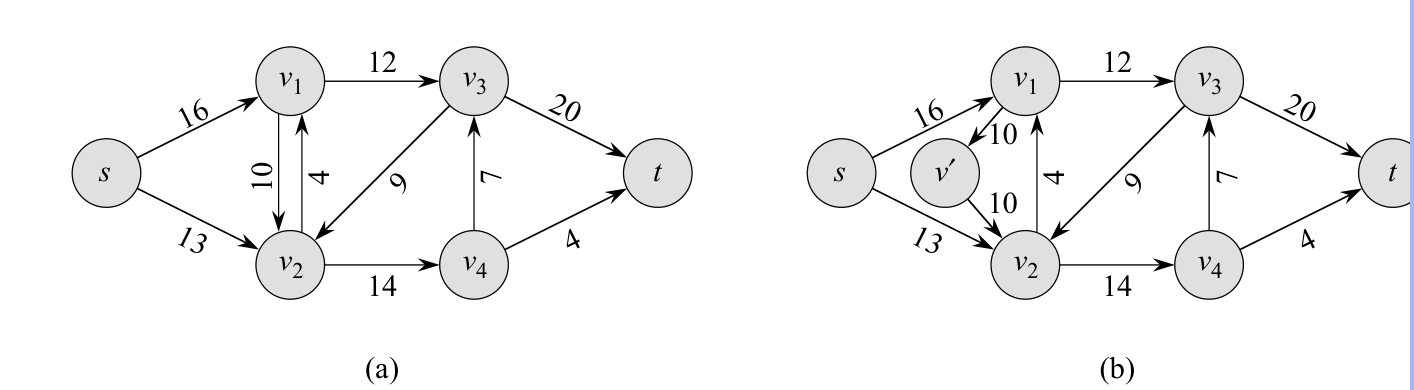
\includegraphics[width=0.8\linewidth]{img/image_2022-11-18-14-50-34.png}
	\caption{A network with antiparallel (reverse) edges ($ v_1 \to v_2 $)}
	\label{fig:358:antiparallel}
\end{figure}


Antiparallel edges can be handled by building an equivalent network with no antiparallel edges (See:~\ref{fig:358:antiparallel}) via splitting an antiparallel edge into a new vertex and two edges.

\begin{figure}[H]
	\centering
	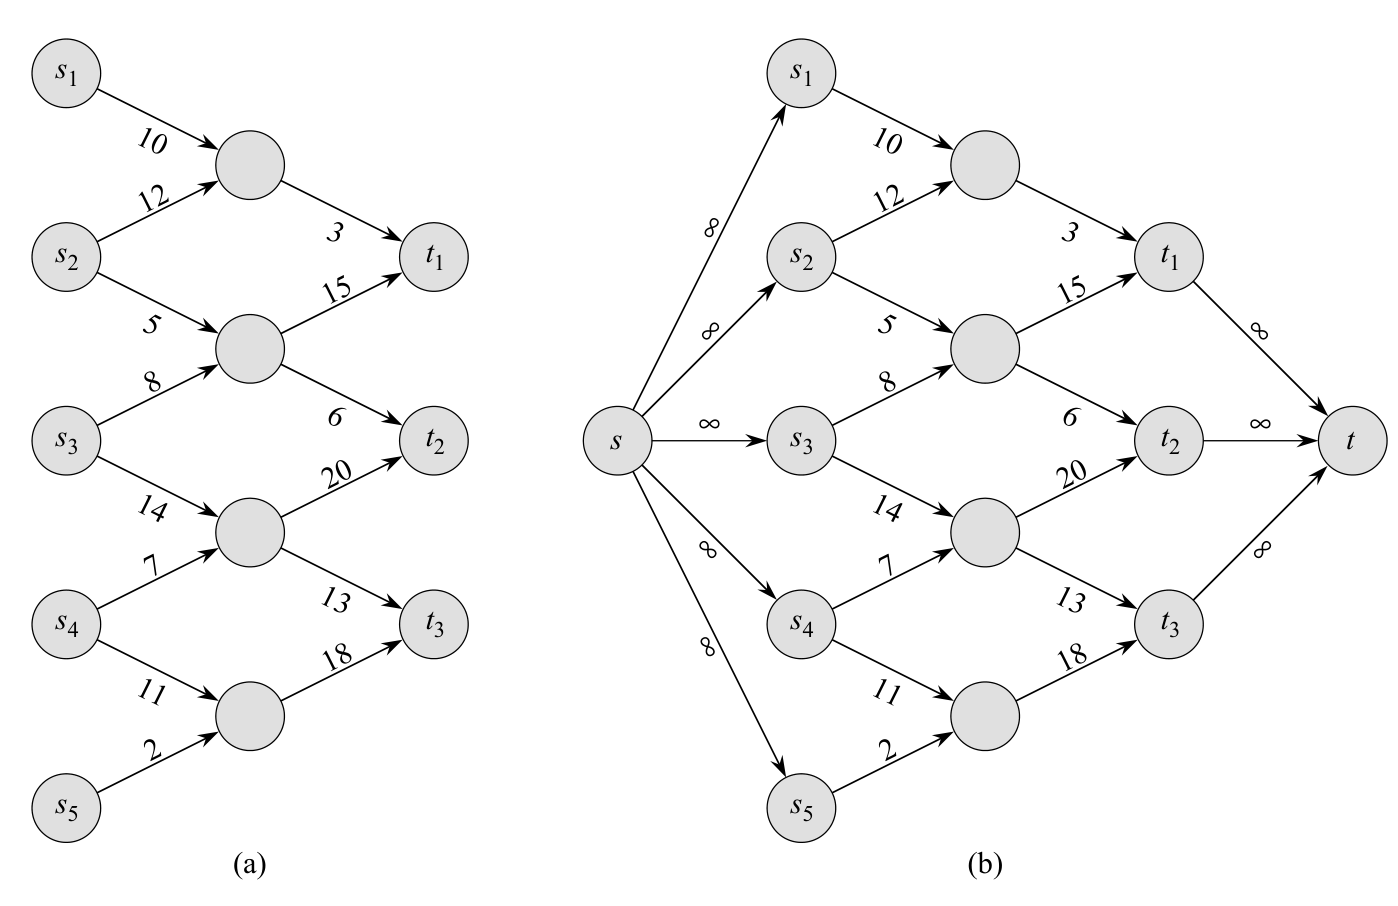
\includegraphics[width=0.8\linewidth]{img/image_2022-11-21-13-12-11.png}
	\caption{Multiple sources \& sinks}
	\label{fig:358:supersourcesink}
\end{figure}

Multiple sources and sinks can be modelled by attaching a \textbf{supersource} and \textbf{supersink} with infinite capacity between each of the existing sources and sinks (\ref{fig:358:supersourcesink}).



One method for solving the maximum flow problem is the \textbf{Ford-Fulkerson} method\mn{It actually encompasses a number of implementations with different runtimes}



\begin{definition}

	\begin{codebox}
	\Procname{$\proc{FORD-FULKERSON-METHOD}(G, s, t)$}
	\li $ f \gets 0 $
	\li \While $ \exists $ augmenting path $p \in$ residual network $G_f$ \Do 
	\li 	augment flow $ f $ along $ b $ \End
	\li \Return $ f $
	\end{codebox}
	
\end{definition}

\begin{definition}
	\textbf{Residual networks} $ G_f $ are graphs that represents the how much we can still change the flow on the edges of $ G $, i.e $ c_f(u,v) = c(u,v) - f(u,v) $. If this capacity is negative the edge is omitted from the residual network.
	Note that it may be sometimes necessary to send back flow along an edge (or decreasing the flow along an edge).
	The maximum amount of backflow that can be supported along the edge $ (u,v) $ is the current flow along the edge.
	This can be accomplished by adding a new edge in the opposite direction $ (v,u) $ with capacity equal to $ f(u,v) $

	So, more formally,

	\begin{equation}
		c_f(u,v) = \begin{cases}
			c(u,v) - f(u,v) & \text{if } (u,v) \in E \\
			f(v,u) & \text{if } (v, u) \in E \\
			0 & \text{otherwise}
		\end{cases}
	\end{equation}

\end{definition}

The \textbf{augmentation} of flow $ f $ by $ f' $, $ f \uparrow f' $ is given by

\begin{equation}
	(f \uparrow f')(u,v) = \begin{cases}
		f(u,v) + f'(u,v) - f'(v,u) & \text{if } (u,v) \in E \\
		0 & \text{otherwise}
	\end{cases}
\end{equation}

\begin{lemma}
	$ f \uparrow f'$ is a flow in $ G $ with value $ |f+f'|= |f| + |f'| $
\end{lemma}

\begin{lemma}
	Flow is conserved, i.e.


	\begin{equation}
		(f\uparrow f') (u, v) = f(u,v) + f'(u,v) - f'(v,u) \le f(u,v) + f'(u,v) \le f(u,v) + c_f(u,v) = c(u,v)
	\end{equation}

	\begin{equation}
		\sum_{}^{v\in V} (f \uparrow f') (u, v) = 
		\sum_{}^{v\in V} (f \uparrow f') (v, u)
	\end{equation}
	
	
\end{lemma}




\begin{definition}
	An \textbf{ augmenting path} $ p $ is a simple path from $ s $ to $ t $ in the residual network $ G_f $.

\end{definition}





\begin{definition}
	The \textbf{Edmonds-Karp} algorithm is an instance of the Ford-Fulkerson method that chooses the shortest (in terms of edge count) augmenting path using BFS and can be show to terminate after $ O(VE) $ augmentations and has $ O(VE^2) $ runtime (since BFS is $ O(V+E) $)

	Suppose $ p $ is a path.

	\begin{equation}
		C_p(p) = min \{ c_f(u,v) : (u,v) \text{ on path } p \} 
		\end{equation}

\end{definition}

\section{Theory of Computation}

\subsection{Finite Automata}

\begin{definition}
	\textbf{Deterministic Finite Automata (DFAs)}\mn{Glorified if-statements}

	Given a sequence of inputs they can accept (true) or reject (false).

	More technically, a DFA is a 5-tuple $ (Q, \Sigma, \delta, q_0, F) $ where



		\begin{itemize}
			\item A set of states $ Q $
			\item An input alphabet $ \Sigma $ (domain of input)
			\item Transition function $ \delta : Q \times \Sigma \to Q $ which takes in a state and some input $ \in \Sigma $ to transition to some other state
			\item An initial state $ q_o \in Q $
			\item A set of accepting states $ F \subseteq Q $
		\end{itemize}

\end{definition}

\begin{example}
		Create a DFA that accepts strings of the form \texttt{"abc"}
		\begin{figure}[H]
			\centering
			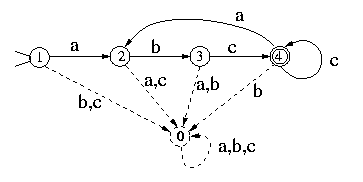
\includegraphics[width=0.8\linewidth]{img/image_2022-11-24-16-18-31.png}
			\caption{Note non-accepting state 0 w/ loop. Accepting state $ q_3 $ indicated via double circle}
		\end{figure}
\end{example}

\begin{example}
	Create a DFA that accepts all inputs with an even number of 0s. $ \Sigma = \{0\}  $


	\begin{equation}
		q_0 \xleftrightarrow{0} q_1
	\end{equation}

	where $ q_0 $ is the accepting state
\end{example}


\begin{example}
	Create a DFA on binary strings that only accepts on strings with a number of 0s that is a multiple of 3

	\begin{figure}[H]
		\centering
		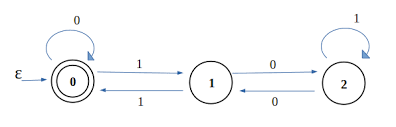
\includegraphics[width=0.8\linewidth]{img/image_2022-11-24-16-25-14.png}
	\end{figure}
	




\end{example}



\begin{definition}
	\textbf{Non-deterministic Finite Automata (NFA)} 

	These are the same as DFAs except we can take an additional input $ \varepsilon $ which is the empty string. On $ \varepsilon $ the NFA branches and computes each branch in parallel. If \textit{any} branch reaches an accepting state the NFA accepts.
\end{definition}


\begin{example}
	Create an NFA that accepts on any input with either a multiple of 2 or 3 0s.
	This is simply the two DFAs we found earlier connected via a branch on $ q_0 $.

\end{example}

\begin{example}

	Find a NFA that accepts on either an even number of 0s or exactly two 1s
	\begin{figure}[H]
		\centering
		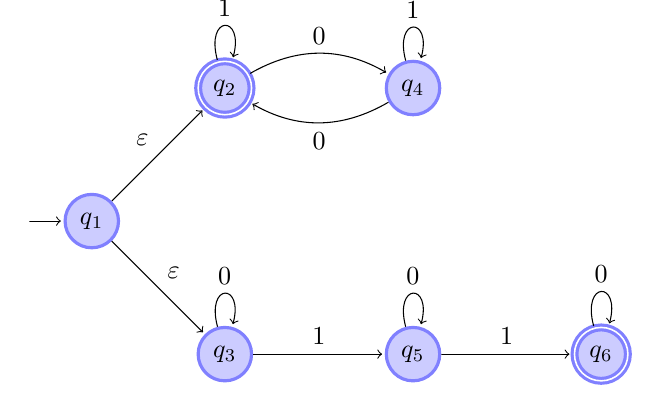
\includegraphics[width=0.8\linewidth]{img/image_2022-11-24-16-32-34.png}
		\caption{Note how this is just two DFAs connected together}
	\end{figure}
\end{example}


\begin{theorem}
	All NFAs can be converted to an equivalent DFA\mn{NFA doesn't provide any additional computability}
\end{theorem}


DFAs and NFAs are memoryless, for example a DFA or NFA is incapable of accepting on a string e.x

\begin{equation}
	O^n I^n \qquad for \qquad n \ge 0
\end{equation}
\marginnote{sequences like \texttt{000111} for n = 3, etc}

\subsection{Turing Machines}

In order to address this Turing machines were introduced. They are basically just a DFA with infinite memory (commonly represented as a tape)

\begin{figure}[H]
	\centering
	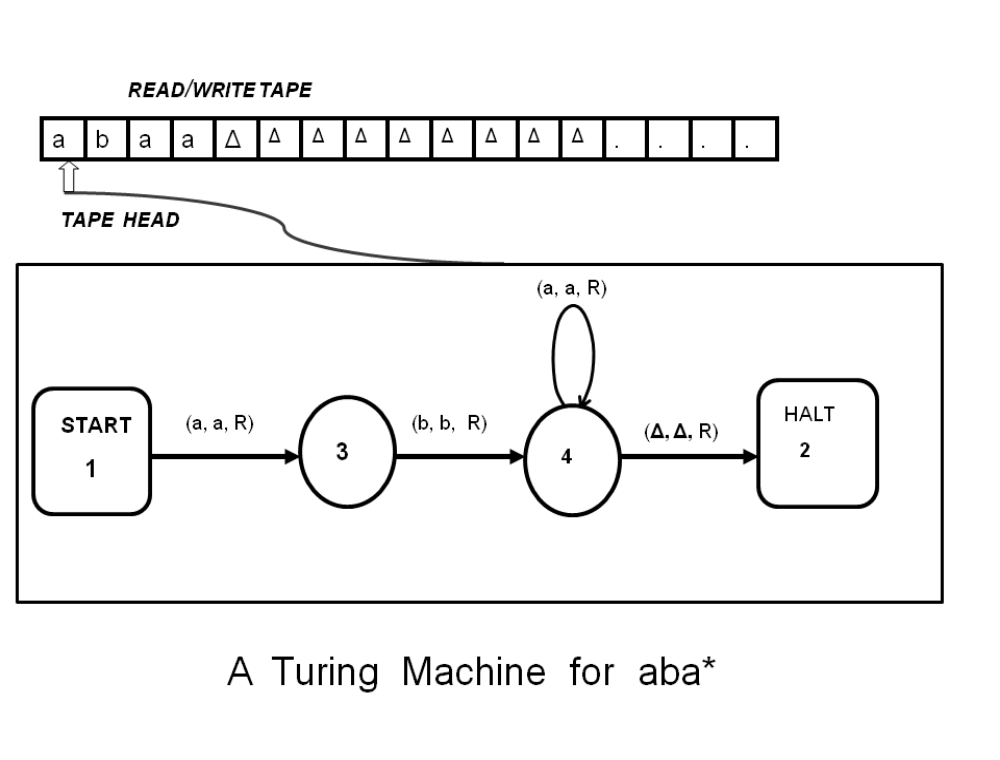
\includegraphics[width=0.8\linewidth]{img/image_2022-11-25-20-18-39.png}
	\caption{A Turing machine for aba}
\end{figure}

Turing machines can compute anything\mn{except for some things like the halting problem etc. TLDR if a problem is not computable by turning machine it is not computable by any finite means. E.g. printing all real numbers between 0 to 1; this is an uncountable infinity but the turning machine tape is countable; larger infinity}



\begin{definition}
	\textbf{Nondeterministic Turing Machine (NTM)}

	Or: a turing machine with a NFA head. Like how a DFA can be converted into a NFA (which would be faster because of parallel computation), a NTM has much better complexity compared to a regular TM.

\end{definition}



\subsection{Complexity Classes}


\begin{definition}
	\textbf{Complexity Classes}

	\begin{itemize}
		\item $ P $: \textbf{P}olynomial number of steps to compute on a TM
		\item $ NP $: Non-deterministic Polynomial: takes a polynomial number of steps to compute on a NTM.
	\end{itemize}

\end{definition}


\begin{theorem}
	All problems in $ NP $ can be verified on polynomial time on a TM, since verifying is like going backwards; since when computing one has to go through all branches on a NTM but when verifying we only have to take one path. 
\end{theorem}



\subsection{NP Completeness}

\begin{blockquote}
	TLDR: NP Completeness 
\end{blockquote}










\begin{definition}
	\textbf{Reductions} 


	\begin{equation}
		A \leq_p B
		\label{eq:358:reduction}
	\end{equation}

	\eqref{eq:358:reduction} means that $ A $ is \textit{polynomially reducible} to $ B $.
	There are about seven equivalent ways to interpret this.

	\begin{enumerate}
		\item There exists a polynomial time function $ f $such that $ \alpha \in A \Leftrightarrow f(\alpha) \in B $
			\begin{itemize}
				\item The contrapositive can also apply; $ f(\alpha) \notin B \Rightarrow \alpha \notin A $
				\item If we can solve it in $ B $-space then we can solve it in $ A $-space
			\end{itemize}
		\item We can decide $ B $ $ \Leftrightarrow $ we can decide $ A $, i.e. that $ A $ 

			\marginnote{\textbf{Hard}: Takes a long time to compute }
		\item Runtime of $ A  \le \text{ runtime } B + O(n^k)$ (some polynomial factor)
	\end{enumerate}

	Reductions will be used



\end{definition}





\begin{definition}
	\textbf{NP-Complete}

	A decision problem $ L $ s.t. $ L \in NP $ such that
	\marginnote{Informally, a problem is NP-Complete if it is at least as hard as any other problem in NP}

	\begin{enumerate}
		\item $ L \in NP $
		\item $ L' \le_p L $ for all $ L'  \in NP $ (NP-hard)
	\end{enumerate}

	Suppose $ A \leq_p B \Rightarrow A \leq B + O(n^k) $

\begin{equation}
	\begin{split}
		\text{if } B \in P & \Rightarrow A \in P  \\
		\text{if } A \in P & \Rightarrow B \in ?  \\
		\text{if } B \in NPC & \Rightarrow A \in ?  \\
		\text{if } A \in NPC & \Rightarrow L' \le_p A \le_p B \Rightarrow B \in NP\text{-hard } \\
	\end{split}
\end{equation}


\end{definition}

\subsubsection{Solving NPC Problems}

Given some decision problem $ A $
\begin{enumerate}
	\item Showing $ A \in NP$
		\begin{itemize}
			\item Provide a \textit{certificate} of $ A \in NP $: the evidence that the problem is an instance of $ A $
			\item Provide a \textit{verification procedure} to check of the certificate is really an instance of $ A $
			\item Argue why the verification procedure is polynomial time
		\end{itemize}
	\item Showing $ A \in NP\text{-hard} $
		\begin{itemize}
			\item Determine which NPC problem $ L' $ we will use (usually provided on exam)
			\item Show that $ L' \le_p A$; transform a known NPC problem to an unknown (i.e. NP-hard)
		\end{itemize}
\end{enumerate}

Showing that $ A $ is NP-Complete requires proving both of the above.






\begin{example}

	\begin{itemize}
		\item Ham-Cycle: Given $ G = (V,E) $, find a simple \textit{cycle} that travels through all vertices.
		\item Ham-Path: Given $ G = (V,E) $, find a simple \textit{path} that travels through all vertices.
	\end{itemize}


	1. Show that Ham-Cycle is in NP

	\begin{itemize}
		\item \textbf{Certificate}: a cycle $ C = \{v_0, v_1 \ldots v_n \}  $
		\item \textbf{Verification}: 
			\begin{itemize}
				\item Check that all of the edges in the cycle are in the graph; $ \forall i, (v_i, v_{i+1}) \in E$. This is $ O(VE) $
				\item Check that all vertices appear exactly once $ O(V) $
				\item This verification procedure is clearly of polynomial time
					\marginnote{Proof can be fairly hand wavy for these simple complexities}
			\end{itemize}

	\end{itemize}

	2. Show that Ham-Cycle $ \in $ NP-hard via Ham-Path


	\begin{equation}
		\text{Ham-Path} \le_p \text{Ham-Cycle}
	\end{equation}

	We note that we can transform the known NPC problem (that we proved in the previous part of this example) into an unknown by adding an additional vertex $ x $ to $ G $ to form $ G' $. Then, for each vertex $ v $ of $ G $, add an edge to $ (v, x) $. This will guarantee forming a ham-cycle.

	Construct $ G' = (V', E') $, $ V' = V \cup {x}  $

	\begin{equation}
		E' = E \cup {(v,x), (x,v) | v \in V}
	\end{equation}

	Claim: $ <G> \in\text{Ham-Path} \Leftrightarrow <G'> \in \text{Ham-Cycle}$


	\begin{itemize}
		\item $ \Rightarrow $ proof: Suppose $ G $ is an instance of Ham-Path ($ \exists V = v_o \to v_1 \to v_n  \in G $), therefore $ x \to v_0 \to v_1 \to v_n \to x$ is a ham-cycle in $ G $. So $ G' $ is an instance of a ham-cycle
		\item $ \Leftarrow $ proof: Suppose $ G' $ is an instance of Ham-Cycle, then $ \exists v_0 \to v_1 \to  v_n \to  x \to  v_0 $; a known cycle in $ G' $
		\item We can remove $ x $ to form a ham-path in $ G $
		\item And therefore $ G $ is an instance of ham-path
	\end{itemize}
	
\end{example}


\begin{definition}
	\textbf{Combinatorial Equivalence Checking} 


	Given boolean formulas $ A(x_1, x_2, x_3 \ldots x_n) $ and  $  B(x_1, x_2, x_3 \ldots x_n)  $, does there exist an assignment such that $ A \neq B $?

	\texttt{Formula-SAT}: Given a boolean formula $ F(y_1, \ldots y_k) $, is there an assignment such that $ F = 1 $?


\end{definition}


\begin{example}
	1) $ CEC \in NP $. 

	\begin{itemize}
		\item Certificate: assignment $ x_1, \ldots x_n $
		\item Verification: Evaluate $ A, B $ and check if $ A \neq B $
	\end{itemize}

	2) $ CEC \in NP $-hard via Formula-SAT

	\begin{equation}
		\text{Formula-SAT} \le_p \text{CEC}
	\end{equation}

	Given a boolean formula $ F $, construct $ A = F $ and $ B = 0 $. Then, makke a claim that $ <F> \in Formula-SAT \Leftrightarrow <A,B> \in CEC $.


	\begin{itemize}
		\item $ \Rightarrow $ proof: there exists an 
	\end{itemize}

	
	




\end{example}


\begin{example}

	Prove that Half-3-CNF-SAT is NP-Complete. Given a 3-CNF formula $ \Phi $ with $ n $ variables and $  m $ clauses, does there exists a truth assignemnt to $ \Phi $ that causes exactly $ m/2 $ of the clauses to evaluate to true and exactly $ \frac{m}{2} $ of the clauses to evaluate to false. Now that $ \Phi  $ can contain duplicate clauses and tautological classes like $ x \lor \neg x \lor y  $


	1: Show that Half-3-CNF-SAT is in NP

	Certificate: an assignment of true, false sequence to $ \Phi $.
	Verification: evaluate all clauses and make sure exactly half are $ 1 $ and the other half is $ 0 $. This is $ O(m) $


	2: Show that Half-3-CNF-SAT is NP-hard via 3-CNF-SAT

	\begin{equation}
		\text{3-CNF-SAT} \le_p \text{Half-3-CNF-SAT}
	\end{equation}

	Attempt: construct $ \Phi' = \Phi \land (p\lor q \lor r )^m$. This is incorrect.

	Attempt: construct

	\begin{equation}
		\Phi' = \Phi \land (p \lor q \lor r )^m \land (p \lor q \lor r )^{2m}
	\end{equation}

	Claim: 
	\begin{equation}
		<\Phi> \in 3-SAT \Leftrightarrow <\Phi'> \in Half-3-CNF-SAT
	\end{equation}
	
	


	
	




	
\end{example}


\begin{example}
	Graph-3-colourability: Given $ G=  (V,E) $, can you assign one of three colours to each vertex such that no two adjacent vertices have the same colour?


	k-clique-cover: Given $ G = (V,E) $ and $ k $, can we partition the vertices $ v $ into $ v_1, \ldots v_k $ such that each $ v_i $ is a clique. This is known to be NP-Hard


	1) Certificate: an assignment of colours to edge vertices. Verification: iterate over each edge and check that the vertices on each end of the vertex are not of the same colour.

	2) 3-col is NP-hard via k-clique-cover. In particular we will do this via 3-clique-cover

	\begin{equation}
		3-clique-cover \le_p 3-col
	\end{equation}

	Given $ G = (V,E) $ is an instance of 3-clique-cover, construct $ G' = (V', E') $ is the complement of $ G$ -- $ V' = V $, $ E' = \{(u,v)| (u,v) \notin E\} $. \mn{Note that this is in polynomial time. Remember to put this on the solution for exams!}

	Claim: 

	\begin{equation}
		<G> \in 3-clique-cover \Leftrightarrow <G'> \in 3-col
	\end{equation}

	Forwards: suppose $ G $ has a 3-clique-cover. So then we color each set $ v_i $ a different color. Then $ u.color = v.color \Rightarrow (u,v,) \in E \Rightarrow (u,v) \notin E' $.
	So $ G $ is 3-colourable

	Backwards: suppose $ G' $ is 3-colourable. $ \exists $ coloring such that $ u.color = v.color \Rightarrow (u,v,) \notin E' \Rightarrow (u,v) \in E $. Therefore let all nodes of the same color be a clique; G.



\end{example}


\begin{example}
Partition: Let $ P $ be a set of positive integers. $ P $ is an instance of Partition if 

\begin{equation}
	\exists P_1, P_2 \subseteq P \text{ such that } P_1 \cup P_2 = P \text{ and } \P_1 \cap P_2 = \{\} \text{ and }  \sum_{x \in P_1} x = \sum_{x \in P_2} x.
\end{equation}

Subset-sum: Given a set of positive integers $ X $ and positive integer $ t$, does there exist

$ S' \subseteq S $ s.t. $ \sum S' = t $



Showing that this is NP is fairly trivial so we'll skip it. Showing that it is NP-hard is trickier.

We will take the approach of showing that Partition is NP-Hard via Subset-sum


\begin{equation}
	\text{Subset-sum} \le_p \text{Partition}
\end{equation}

Given set $ S $ and target $ t $, construct $ x = \sum S $, $ P = S \cup \{x-2t\}  $.

Claim: 

\begin{equation}
	<s,t> \in subset-sum \Leftrightarrow <P> \in Partition
\end{equation}

Forwards: Suppose $ \exists T_1 \subseteq A \text{ st. } \sum T_1 = t $. Let $  $


	
\end{example}




% 358 END
\end{document}



























